\newcommand{\mypapersize}{A4}
%% e.g., "A4", "letter", "legal", "executive", ...
%% The size of the paper of the resulting PDF file.

\newcommand{\mylaterality}{oneside}
%% "oneside" or "twoside"
%% Either you are creating a document which is printed on both, left pages
%% and right pages (twoside) or you create a document which is printed
%% on right pages only (oneside).

\newcommand{\mydraft}{false}
%% "true" or "false"
%% Use draft mode? If true, included graphics are replaced by empty
%% rectangles (of same size) and overfull boxes (in margin space) are
%% marked with black box (-> easy to spot!)

\newcommand{\myparskip}{half}
\setlength{\parindent}{2em}
%% e.g., "no", "full", "half", ...
%% How to separate paragraphs: indention ("no") or spacing ("half",
%% "full", ...).

\newcommand{\myBCOR}{0mm}
%% Inner binding correction. This value depends on the method which is
%% being used to bind your printed result. Some techniques do not
%% require a binding correction at all ("0mm"), other require for
%% example "5mm". Refer to KOMA script documentation for a detailed
%% explanation what a binding correction is and how to measure it.

\newcommand{\myfontsize}{12pt}
%% e.g., 10pt, 11pt, 12pt
%% The font size of the main text in pt (points).

\newcommand{\mylinespread}{1.0}
%% e.g., 1.0, 1.5, 2.0
%% Line spacing in %/100. For example 1.5 means 150% of the usual line
%% spacing. Please use with caution: 100% ("1.0") is fine because the
%% font was designed for it.

\newcommand{\mylanguage}{ngerman,american}
%% "english,ngerman", "ngerman,english", ...
%% NOTE: The *last* language is the active one!
%% See babel documentation for further details.


%% Name of the biblatex file that holds the references.

\newcommand{\mydispositioncolor}{0,0,0}

%% e.g., "30,103,182" (blue/turquois), "0,0,0" (black), ...
%% Color of the headings and so forth in RGB (red,green,blue) values.
%% NOTE: if you are using "0,0,0" for black, printers might still
%%       recognize pages as color pages. In case this is a problem
%%       (paying for color print-outs vs. paying for b/w-printouts)
%%       please edit file "template/preamble.tex" and change
%%       "\definecolor{DispositionColor}{RGB}{\mydispositioncolor}"
%%       to "\definecolor{DispositionColor}{gray}{0}" and thus
%%       overwriting the value of \mydispositioncolor above.

\newcommand{\mycolorlinks}{true}  %% "true" or "false"
%% Enables or disables colored links (hyperref package).

\newcommand{\mytitlepage}{template/title_Thesis_TU_Graz}

%% Your own or one of following pre-defined title pages:
%% "template/title_plain_maketitle": simple maketitle page
%% "template/title_Diplomarbeit_KF_Uni_Graz.tex": fancy (german) title page for KF Uni Graz
%% "template/title_Thesis_TU_Graz":
%%             titlepage for Graz University of Technology (correct
%%             (old?) Corporate Design) by Karl Voit (2012)
%% "template/title_Thesis_TU_Graz_-_kazemakase":
%%             titlepage for Graz University of Technology
%%             (correct new Corporate Design) by kazemakase (2013):
%%             see https://github.com/novoid/LaTeX-KOMA-template/issues/5
%% "template/title_VWA": titlepage for Vorwissenschaftliche Arbeit


%% Load main settings for document preamble:
\input{template/preamble}%% DO NOT REMOVE THIS LINE!


\setboolean{english_affidavit}{true}  %% "true" or "false"
%% If set to "true": the language of the statutory declaration text is set to
%% English, otherwise it is in German.


%% ========================================================================
%%%% Document metadata
%% ========================================================================

%% general metadata:
\newcommand{\myauthor}{Ramez Maher Abdalla}  %% also used for PDF metadata (hyperref)
\newcommand{\myauthorwithexistingtitles}{\myauthor, MSc}  %% including
                                %% university degree already held
                                %% (BSc, MSc, ...)
\newcommand{\mytitle}{Applying Data Analytics Framework For Subsurface Energy Production Systems }  %% also used for PDF metadata (hyperref)
\newcommand{\mysubject}{WITH FOCUS ON PREDICTIVE MENTAINANCE, MULTIPHASE FLOW ESTIMATION AND PRODUCTION OPTIMIZATION}  %% also used for PDF metadata (hyperref)
\newcommand{\mykeywords}{KEYWORDS}  %% also used for PDF metadata (hyperref)

%% this information is used only for generating the title page:
\newcommand{\myworktitle}{Doctor of Philosophy}  %% official type of work like ``Master theses''
\newcommand{\mygrade}{Dr.-Ing.} %% title you are getting with this work like ``Master of ...''
\newcommand{\mystudy}{Subsurface Energy Production Systems} %% your study like ``Arts''
\newcommand{\mydegreeprogramme}{Doctoral Program: \mystudy} %% Master's or PhD degree programme
\newcommand{\myuniversity}{Clausthal University of Technology} %% your university/school
\newcommand{\myinstitute}{Institute of subsurface energy systems} %% affiliation
\newcommand{\myinstitutehead}{Prof. Dr. Leonhard Ganzer} %% head of institute
\newcommand{\mysupervisor}{Prof. Dr. Philip Jaeger} %% your supervisor
\newcommand{\mycosupervisor}{Prof. Dr. Co-supervisor}
\newcommand{\mysubmissionmonth}{December} %% month you are handing in
\newcommand{\mysubmissionyear}{2022} %% year you are handing in
\newcommand{\mysubmissiontown}{Clausthal} %% town of handing in (or \myhometown)

%% additional information for generic_documentation title page
\newcommand{\myid}{1234567} %% Matrikelnummer
\newcommand{\mylecture}{LECTURE} %%


%% ========================================================================
%%%% MISC command definitions
%% ========================================================================
\input{template/mycommands}

%% ========================================================================
%%%% Typographic settings
%% ========================================================================
\input{template/typographic_settings}


%% ========================================================================
%%%% MISC usepackages
%% ========================================================================

%% ... it's OK to put here your own usepackage commands ...
%test

\usepackage{soul}
\usepackage{booktabs}
\usepackage{amsmath}
\usepackage{placeins}
\usepackage{geometry}
\usepackage{booktabs}
\usepackage{tabularx,siunitx}
\usepackage{algorithm}
\usepackage{algpseudocode}
\geometry{a4paper, portrait, tmargin=1.5in, bmargin=1.5in, outer=1.5in}
\usepackage{tikz}
\usepackage{nomencl}
%% ========================================================================
%%%% MISC self-defined commands and settings
%% ========================================================================

%% ... it's OK to put here your own newcommand/newenvironment-definitions ...




\newcommand{\myLaT}{\LaTeX{}@TUG\xspace} %% LaTeX@TUG text "logo"

\hyphenation{ex-am-ple hy-phen-ate}  %% in order to use German umlauts
%% here (Ver-\"of-fent-li-chung), you have to check for
%% activated \usepackage[T1]{fontenc} in the preamble

%% override default language of babel: (be sure to know, what you're
%% doing here)
%\selectlanguage{american}
%\selectlanguage{ngerman}

%% ========================================================================
%%%% Templates
%% ========================================================================

%% template for inserting figures:
% \myfig{}%% filename
%       {}%% width/height
%       {}%% caption
%       {}%% optional (short) caption for list of figures
%       {fig:}%% label

%% acronyms in small caps: \myacro{UNESCO}

\input{template/pdf_settings}  %% should be *last* definitions in preamble!
%% ========================================================================
%%%% begin{document}
%% ========================================================================
\begin{document}

\frontmatter                    %% KOMA: roman page numbers and such; only available in scrbook

\input{\mytitlepage}

%%\input{template/declaration_TU_Graz}


%% include the abstract without chapter number but include it on table of contents:
\cleardoublepage
\chapter*{Acknowledgments}

I wish to thank my committee members who were more than generous with their expertise and precious time. A special thanks to Prof. Dr. XXX, my committee chairman and Prof. Dr Philip Jaeger, my thesis main advisor for his countless hours of reflecting, reading, encouraging, and most of all patience throughout the entire process. Their excitement and willingness to provide feedback made the completion of this research an enjoyable experience. Special thanks to my colleagues Dr. Carlos Paz, Dr. Nelson Perozo and Mrs. Hanin Samara for their contributions and support while writing the papers relevant to this thesis.
\chapter*{Abstract}\label{cha:abstract}
This is a placeholder for the abstract. It summarizes the whole thesis
to give a very short overview. Usually, this the abstract is written
when the whole thesis text is finished.

\chapter*{Kurzfassung}\label{cha:abstract_german}
This is a placeholder for the german abstract. It summarizes the whole thesis
to give a very short overview. Usually, this the abstract is written
when the whole thesis text is finished.
\printnomenclature

\clearpage
\section*{Nomenclature} 
\begin{acronym}
    \acro{ESP} {electrical submersible pump}
\end{acronym}
\begin{acronym}
    \acro{SRP}{sucker rod pump}
\end{acronym}
\begin{acronym}
    \acro{XGBoosting}{extreme gradient boosting}
\end{acronym}
\begin{acronym}
    \acro{EOR}{enhanced oil recovery}
\end{acronym}
\begin{acronym}
    \acro{SME}{subject matter experts}
\end{acronym}
\begin{acronym}
    \acro{WAG}{water alternating gas}
\end{acronym}
\begin{acronym}
    \acro{PSO}{particle swarm optimization}
\end{acronym}
\begin{acronym}
    \acro{PCA}{principle component analysis}
\end{acronym}
\begin{acronym}
    \acro{VFM}{virtual flow meter}    
\end{acronym}
\begin{acronym}
    \acro{NPV}{net present value}    
\end{acronym}
\begin{acronym}
    \acro{RL}{reinforcement learning}    
\end{acronym}
\begin{acronym}
    \acro{FRQ}{pump frequency}
\end{acronym}

\begin{acronym}
    \acro{PDP}{pump discharge pressure}
\end{acronym}

\begin{acronym}
\acro{PIP}{pump intake pressure }    
\end{acronym}

\begin{acronym}
\acro{WHP}{well head pressure}    
\end{acronym}

\begin{acronym}
\acro{WHT}{well head temperature}    
\end{acronym}

\begin{acronym}
\acro{MT}{motor temperature }    
\end{acronym}

\begin{acronym}
\acro{CHP}{casing head pressure}    
\end{acronym}

\begin{acronym}
\acro{Current}{variable speed drive output current}    
\end{acronym}

\begin{acronym}
\acro{MDHF}{motor downhole failures}    
\end{acronym}

\begin{acronym}
\acro{EDHF}{electrical downhole failures}    
\end{acronym}

\begin{acronym}
\acro{ROC}{receiver operating characteristics}
\end{acronym}


\begin{acronym}
\acro{CNN}{convolutional neural network}
\end{acronym}


\begin{acronym}
\acro{LSTM}{long short term memory algorithm}
\end{acronym}
\clearpage
\tableofcontents


\listoffigures

\listoftables

\mainmatter                     %% KOMA: marks main part using arabic page numbers and such; only available in scrbook

\chapter{Introduction}

As the digital energy field is expanding quickly, The amount of data stored is growing exponentially. With this surge, the role of data analytics has become a hugely important through the whole subsurface energy fields sectors (i.e. upstream and downstream). As the fields of big data analytics, artificial intelligence and machine learning grow, companies need data analysis in various forms and sectors through their chain. This makes potential use of data mining methodologies to learn from experts how they predict well failures. The performance can be dramatically improved by successful failure predictions either by adjusting operating parameters to forestall failures or by scheduling maintenance to reduce unplanned repairs and to minimize downtime. In the smart subsurface energy fields, the measurements from fields are used for efficient and integrated management. Hence machine learning and data analytics researches increased drastically.

Machine learning in the oil and gas industry can be divided into three main categories. Those are either extracting knowledge from data in real-time form, predictive analytics and production optimization through real data. As aforementioned, the oil and gas industry generates enormous data. However, there is no full usage of that data. With the help of machine learning, this data can be processed to make real time diagnostic applications. Furthermore, machine learning can help to make predictions regarding how oil production from wells. Also, it could help in optimizing production through identifying the most efficient ways to set up production systems. Such applications can include advisory systems for injection rates, pumping stroke per minutes and anything determining optimal well spacing, deciding where to drill, and testing different techniques for fracking.

These three categories exhibit how machine learning can help oil and gas companies make better decisions today and plan for the future based on past data. This will be critical as they face the challenges of improving their workflow while adapting to new technologies. From energy systems perspective, there are several areas where machine learning can be applied to help improve oil and gas industry workflows, including: Real-time drilling, reservoir engineering, Oil and gas production and procurement, downtime prevention and well testing. Etc

The above application areas include a wide range of tasks that involve oil and gas industry employees. Machine learning can help these employees become more efficient at their jobs, help them make better decisions, and improve the quality of products they produce. However, the transition will not happen overnight. As the oil and gas industry prepares to incorporate machine learning, it is important to recognize the challenges involved. The first significant challenge is the oil and gas industry’s need to hire data scientists qualified to extract knowledge from industry data. This may be difficult for companies that already have a shortage of workers or companies in regions where there aren’t many people with data science skills. 

Another challenge is the large amount of data oil and gas companies deal with daily. This means that the machines doing the analysis will need to be very powerful to process it all in a reasonable amount of time. Finally, training the machine learning algorithms to recognize valuable data patterns for oil and gas companies will require a great deal of time and effort. However, the payoff of accurate models to make data-backed decisions will be worth it for oil and gas companies.

The realization that machine learning techniques can be successfully deployed for oil and gas companies is still occurring across the industry. As more energy companies investigate ML use cases, we will see an increase in its adoption. This will certainly change how oil and gas companies operate, and it is just one example of how data science is changing how we do business.

Oil and gas companies are already using machine learning to help with prediction models, produce better results from their resources, and optimize their processes. Machine learning has the power to revolutionize the oil and gas industry. This forward momentum is crucial for the sector solely responsible for keeping the rest of society moving.

In the coming years, we will see more and more ML technologies used by oil and gas companies around the world. In fact, the future of the oil and gas industry can be found in the convergence of many different technologies, including machine learning. Companies who adapt early can improve their resource optimization and gain a more detailed look at their progress.


This research is prepared to develop applications on the whole framework of data analytics applications on the subsurface energy systems industry. Applications on three stages of data analysis are developed. These three stages are descriptive, predictive and prescriptive analytics. Firstly a virtual flow meters on the electrical submersible pump as an application on descriptive bases. Secondly, predictive maintenance of the electrical submersible pump is developed as an application on predictive analytics. On prescriptive analytics basis, the reinforcement learning is used to provide an optimum policy of steam injection rate.

This thesis is organized into eight chapters. Chapter 1 “Introduction” is prepared to give a general overview about the subject of the present study. Chapter 2 “Literature Review” presents a review for the data analysis and relevant literature on oilfield applications of real time, predictive and prescriptive analytics on petroleum production  systems. It also discussed the applicability of these various approaches. Then, concluding remarks. Chapter 3 “Statement of the Problem, Thesis Objectives and Methodology” describes the statement of the problem and the main objectives of the study and workflow pipeline for each application. Chapter 4 “virtual flow metering” Discussing the data driven multiphase flow estimation through artificial lift systems with focus on electrical submersible pump. Chapter 5 “Predictive modeling” discuss predive maintenance of the electrical submersible pumps by predicting pre-workover events using principle component analysis pipelined with extreme gradient boosting. Chapter 6 “prescriptive analytics” discuss the use of actor critic reinforcement learning to lead decision-making in energy systems optimization and introduces also a proof of value on steam injection optimization. Chapter 7 “Results and Discussion” shows the proposed models accuracy and various matrices used for testing to validate models. Chapter 8 “Conclusion and Recommendations” concludes the thesis results and findings. In addition, it presents the recommendations for the future research work in this topic.

\chapter{Background and Related Work}

\section{Introduction}


\section{Mapping production and reservoir data}


\begin{table}[]
\resizebox{\textwidth}{!}{%
\begin{tabular}{|l|lll|}
\hline
Data   Categories & \multicolumn{3}{l|}{Production  Engineering Component}                                                                                              \\ \hline
Static Data &
  \multicolumn{1}{l|}{\begin{tabular}[c]{@{}l@{}}Wellbore   Data Completion\\    \\ Class A\end{tabular}} &
  \multicolumn{2}{l|}{\begin{tabular}[c]{p{8cm}}Tubing Size,\\ Artificial Lift used with   its relevant characteristics\\ pump type and its   characteristic curve\\ Perforation Depth\end{tabular}} \\ \hline
Depth Data &
  \multicolumn{1}{l|}{\begin{tabular}[c]{@{}l@{}}Fluid Properties\\    \\ Class B\end{tabular}} &
  \multicolumn{2}{l|}{\begin{tabular}[c]{p{8cm}}Produced Fluid Data,\\ Interfacial Tension\\ Formation Volume Factor\\Density\\  Viscosity\end{tabular}} \\ \hline
\multirow{2}{*}{Time Data} &
  \multicolumn{1}{l|}{\multirow{2}{*}{\begin{tabular}[c]{@{}l@{}}Operating   Parameters\\    \\ Class C\end{tabular}}} &
  \multicolumn{2}{l|}{\begin{tabular}[c]{p{8cm}}It depends on well   completion (Gas Lift, Electrical Submersible Pumps, Sucker Rod Pumps, Natural   Flow, Gas Nat. Flow, Plunger Lift…). These parameters could me controlled parameters, manipulated paramters or disturbance paramters\\   Example \ac{ESP}:\\ Pump head\\ Motor temperature\\Frequency\\ Voltage\\ …\end{tabular}} \\ \cline{3-4}  \hline
\end{tabular}%
}
\caption{}
\label{production data}
\end{table}


\begin{table}[]
\resizebox{\textwidth}{!}{%
\begin{tabular}{@{}|l|ll|@{}}
\toprule
Data Categories &
  \multicolumn{2}{l|}{Reservoir Engineering   Component} \\ \midrule
\multirow{4}{*}{\begin{tabular}[c]{@{}l@{}}Reservoir Characteristics Data\\    \\ Class A\end{tabular}} &
  \multicolumn{1}{l|}{Geophysical data} &
  \begin{tabular}[c]{@{}l@{}}Seismic survey data\\    Well log data\end{tabular} \\ \cmidrule(l){2-3} 
 &
  \multicolumn{1}{l|}{Petrophysical data} &
  \begin{tabular}[c]{@{}l@{}}Permeability distributions\\    \\ Porosity distributions\\    \\ Formation Depth\\    \\ Reservoir Pressure\\    \\ Reservoir Temperature\\    \\ Fluid contact\end{tabular} \\ \cmidrule(l){2-3} 
 &
  \multicolumn{1}{l|}{Fluid Properties} &
  \begin{tabular}[c]{@{}l@{}}Fluid Composition\\    \\ PVT data\end{tabular} \\ \cmidrule(l){2-3} 
 &
  \multicolumn{1}{l|}{Rock/Fluid interaction data} &
  \begin{tabular}[c]{@{}l@{}}Relative Permeability data\\    \\ Capillary Pressure data\end{tabular} \\ \midrule
\begin{tabular}[c]{@{}l@{}}Project Design Parameters\\    \\ Class B\end{tabular} &
  \multicolumn{2}{l|}{\begin{tabular}[c]{@{}l@{}}Injection/Production well specification\\    \\ Well pattern design\\    \\ Well spacing\\    \\ Well architecture design\\    \\ EOR (Enhanced Oil Recovery) design parameters\end{tabular}} \\ \midrule
\begin{tabular}[c]{@{}l@{}}Field responses data\\    \\ Class C\end{tabular} &
  \multicolumn{2}{l|}{\begin{tabular}[c]{@{}l@{}}Fluid Production data\\    \\ Pressure data\\    \\ Project economics\end{tabular}} \\ \bottomrule
\end{tabular}%
}
\caption{Reservoir Data Categorization}
\label{reservoir_data}
\end{table}

\section{Production engineering applications}
lllllllllllllllllllllllll
fdddddddddddddddd
\section{Reservoir engineering applications}
sdddddddddddddddddddddd
%ToDo: include other sections here.
%\section{Further Content}

\section{Concluding remarks}


\chapter{The objectives \& the data analysis process}

\section{Introduction}
The strategy is to cover data analysis applications over the three main goals. First, descriptive analytics aims to provide insight into what has happened. Second, predictive analytics helps to model and forecast what might happen. Thrird, prescriptive analytics seek to determine the best solution or outcome among various choices, given the known parameters.

Firstly, Pattern recognition applications that use machine learning algorithms to discover various patterns on operating pumping parameters using either supervised or unsupervised algorithms. Afterward, alarms and models are deployed that enables subject matter experts (SMEs) to unleash various behaviors downhole. Inferring real-time measurements using ground-truth values of previous sensors measurements or production tests lies also in this area of research. For instance, the technology of \ac{VFM} is considered one of the main applications in this area. 

The second strategy is predictive analytics. One of the main applications in this area is predictive maintenance. It mainly depends on detecting early signs in sensor measurements that exist by using machine learning and deep learning algorithms. 

Finally, Finally, dive into prescriptive analytics is introduced. It is referred to as the "final frontier of analytic capabilities". prescriptive analytics entails the application of mathematical and computational sciences and suggests decision options. For instance, predicting the optimum operating parameters (ie. pump frequency, injection rate..etc) in order to maximize the \ac{NPV}. Figure ~\ref{fig:Workflow} shows the whole data analytics startgies with their main objectives.  

\begin{figure}
    \centering
    
\includegraphics[keepaspectratio, width=\textwidth]{figures/workflow_design/workflowdesign.png}
    \caption{Workflow design}
    \label{fig:Workflow}
\end{figure}


\section{Objectives}

In the technological terms, this study aims to contribute to the area of data analytics in subsurface energy systems through the development of intelligent computing techniques. The developed applications targets the whole three stages of applications of data analytics. In other words, three different applications would be introduced. These applications are covering descriptive, predictive and prescriptive strategies. They are implemented using machine learning and deep learning algorithms on the oilfield data.

In the scientific terms, the main objective of this work is to develop three  models. First model should be able to predict oil production and water cut on wells that are deployed with electrical submersible pumps. It could be considered as an estimation of multiphase flow rates through wells. Second model would analyze the performance and unleash pattern between pre-event days (i.e. pre-workover days) and pump sensors measurements. The third model would be able to predict the optimum policy for injection rate in steam injection project.Table \ref{tab:workflowtable} presents a Summary of Projects and their relevant objective.

\begin{table}[]
    \centering
    \begin{tabular}{|p{3cm}|c|p{6cm}|}
        \hline
        Project & Area of Research & Objective \\ \hline
        Virtual flow meter for the \ac{ESP} & Descriptive modeling &  Real time inferring of oil rate and water cut of the \ac{ESP} wells using deployed pump sensors measurements \\     \hline
        Predictive maintenance of the \ac{ESP}  & Predictive modeling & Classify abnormal signals from 7 to 10 days before failure using rotated cloud of sensor data projected on principle axes  \\    \hline
        Steam injection rate optimization & Prescriptive modeling & Optimizing injection rate policy over time using actor critic reinforcement learning in order to maximizing the \ac{NPV}\\ \hline
    \end{tabular}
\caption{Summary of Projects and their relevant objective}
\label{tab:workflowtable}
\end{table}
   
\section{The data analysis process}
All of the aforementioned applications follow the process of data analysis applications. Basically all of them include understanding of the data then applying statistics to get insights for an engineering objective. Every study we would encounter is divided into four modules. Each module has a big impact on the overall performance of any problem. These four modules are:
•	Data gathering and exploratory data analysis
•	Feature extraction and transformation
•	Modeling 
•	Testing and Evaluation 

\subsection{Data gathering and exploratory data analysis}
Once the objective is established, A strategy is needed to be created for collecting and aggregating the appropriate data. This data might be quantitative (numeric) data, e.g. pump frequency for \ac{ESP}, stroke per minute for \ac{SRP}, or qualitative (descriptive) data, such as workover failure reason..etc In general, the training data set must include a number of cases from the aforementioned data. Each case contains values for a range of input and output variables.

Next step would be data cleaning. It is a crucial step because it enhance the quality data. Many tasks are included in data cleaning. Those are Removing major errors and duplicates, detecting outliers, and extracting irrelevant observations that have no bearing on the intended analysis. 

Likewise, It is important to carry out an exploratory data analysis. This helps identify initial trends and characteristics, and can even refine the hypothesis. It will give an idea of which inputs are likely to be influential. Exploratory data analysis helps to reveal hidden patterns, correlations, and anomalies using various tools such as visualizations (scatter and box plots, histograms, etc.), dimensionality reduction techniques and sometimes unsupervised algorithms for data grouping.

\subsection{Feature Extraction and transformation}
Feature extraction is one of the keys for a successful pattern recognition application. In definition, feature is a prominent part or characteristic of an object to distinguish itself. In machine learning application, the problem of large input data is encountered. The nature of input paramters could be in wave form or images presented as pixels. In such context, the input data can be transformed into a reduced set of features (also named a features vector). This process is called feature extraction. The selected features are expected to contain the relevant information from the input data. Hence, the desired task can be performed by using this reduced representation instead of the complete initial data.

In essence, feature extraction starts from an initial set of measured data. It builds derived values (features) intended to be informative and non-redundant. This facilitates the subsequent learning and generalization steps. 

\subsection{Modeling}
The type of data analysis is dependant upon the objective of the project. There are many techniques available. Univariate or bivariate analysis, time-series analysis, and regression analysis both linear and logistic could be considered as the fundamental studies for such modeling step. More important is how to apply them. This depends on the data itself and its complexity. Usually less to more complicated algorithms are applied in a sequence in order to unleash patterns inside the data. The inequality of explainability As described in DARPA’s research is that all AI techniques are not created equal in terms of their capacity for explainability. Complex algorithms requires recognition and careful consideration when using them for a particular use case. Figure \ref{fig:ml_explain} maps different types of AI systems according to their learning performance (i.e. accuracy) vs explainability. 

\begin{figure}
    \centering
    
\includegraphics[keepaspectratio, width=\textwidth]{figures/workflow_design/perf_vs_expl.png}
    \caption{Algorithms inequality of explainability}
    \label{fig:ml_explain}
\end{figure}

Broadly speaking, all types of data analysis fit into one of the following three categories. When the data is prepared in desired format, Analytics would be performed which would give the insights for the relationship between sensor measurement, workover events and help in decision making. In these purposes, various algorithms could be used. These algorithms exhabit inverse relation between learning performance and explainability. Algorithms could range from Linear Regression, Clustering, Decision Tree techniques, support vector machines to come to a neural networks and deep neural learning.

\subsubsection{Descriptive analytics for Real time estimation and diagnostic modeling}
The objective of descriptive analysis here is to summarize the past row data to some models. These models are useful because they learn from past behaviors, and understand how they might influence future outcomes. The past row data refers to any point of time that an event has occurred, whether it is one minute ago, or one year ago. For instance, the sensor deployed data can be used to create model infer wells production. 

Diagnostic modeling focuses on understanding why something has happened. It is literally the diagnosis of a problem, just as the \ac{SME}s uses wells data to understand what happened downhole. For instance, it could help identifiying the condition of the sucker rod pump ug dynamomter cards.

\subsubsection{Predictive analytics for predictive maintenance}
Predictive analysis is used to identify future trends and forecasts accurately based on historical data. It has the ability to “predict” what might happen.
It has grown increasingly in recent years due to the evolution of machine learning and deep learning. It is of high importance to oil and gas industry because it helps in increasing production efficiencies through the proactive identification of failure events and the avoidance of deferment losses.

Predictive maintenance is a type of predictive anayltics that uses condition-monitoring sensor data to predict when equipment will fail. By predicting equipment failures, companies can schedule repairs during routine downtime. That enables them avoiding unplanned downtime and production loss. However, in many literature applications the term "predictive maintenance" is used interchangeably to refer to diagnostic modeling or operating data groupping.

Initiative, A key application in oil and geothermal energy systems would be developing an early failure Prediction model for artificial lift systems. In other words to be able to answer the question of when the well is going to fail?

\subsubsection{Prescriptive analytics for optimising manipulating parameters}
The Prescriptive analytics is a relatively new field. These analytics go beyond descriptive and predictive analytics by recommending one or more possible courses of action. It is used to “prescribe” a number of different possible actions and guide them towards an optimum  solution. It supports as advisory systems for the future. This is the final step in the analytics part of the process. It’s also the most complex. This is because it incorporates aspects of all the other analyses that have aforementioned.

Prescriptive analytics is a quite difference in application level. It use a combination of techniques and tools such as simulation studies, computational modelling procedures, and machine learning (ML).

A great example of prescriptive analytics is the algorithms that guide Google’s self-driving cars. Every second, these algorithms make countless decisions based on past and present data, ensuring a smooth, safe ride. Prescriptive analytics also helps in decision making for long term changes in manipulating paramters.

If it is implemented correctly, they could have a large impact on making decisions, and on the company’s bottom line. Technically, such analytics would contribute to the area of production optimization though making decsions on some maniulate parameters such as choke opening, pump frequency, injection rate and pump stroke per minute..etc.

In a nutshell, these analytics are all about providing advice. Prescriptive analytics attempts to quantify the effect of future decisions in order to advise on possible outcomes before the decisions are actually made. 

\subsection{Testing and Evaluation}
Model evaluation is very important in data science. It helps you to understand the performance of your model and makes it easy to present your model to other people. There are many different evaluation metrics out there but only some of them are suitable to be used for regression. This article will cover the different metrics for the regression model and the difference between them. Hopefully, after you read this post, you are clear on which metrics to apply to your future regression model.

Every time when I tell my friends: “Hey, I have built a machine learning model to predict XXX.” Their first reaction would be: “Cool, so what is the accuracy of your model prediction?” Well, unlike classification, accuracy in a regression model is slightly harder to illustrate. It is impossible for you to predict the exact value but rather how close your prediction is against the real value.

// regression modeling

Mean Absolute Error is the average of the difference between the Original Values and the Predicted Values. It gives us the measure of how far the predictions were from the actual output

Mean Squared Error(MSE) is quite similar to Mean Absolute Error, the only difference being that MSE takes the average of the square of the difference between the original values and the predicted values.

The cross plots of predicted versus actual data and calulating R square for this linear model
// classification modeling
The classification methods are evaluated and the best scenario of each algorithm has been chosen. Then, accuracy of each scenario is defined as the ratio of number of correctly classified reviews to the total number of reviews classified by the prediction model. Then, one of the two competitive algorithms was chosen for field applications validation. The results of the precision and recall measured for the proposed classification model is then discussed. This model evaluation is done for each rod pump conditions.

// unsupervised modeling (learning curve and ushape test)
The approach is to compute validation score of each cluster and then combine them in a weighted manner to arrive at the final score for the set of clusters. Let S be a set of clusters {C1 , C2 , C3 ,…………, Cn }, then validity of S will be computed as follows:

Cohesion for a cluster can be computed by summating the similarity between each pair of records contained in that cluster.

Separation between two clusters can be computed by summating the distance between each pair of records falling within the two clusters and both the records are from different clusters.

A set of clusters having high cohesion within the clusters and high separation between the clusters is considered to be good.

In practice, instead of dealing with two metrics, several measures are available which combine both of the above into a single measure. Few examples of such measures are:

Silhouette coefficient
Calisnki-Harabasz coefficient
Dunn index
Xie-Beni score
Hartigan index

Sofar in this blog series, we have looked at how to create automated playlists of songs by clustering a collection of tracks, based purely on their audio features. Previously, we worked on a toy example of 32 songs and showed how Hierarchical Agglomerative Clustering (HAC) can automatically create sub-groups of similar songs. We were able to verify the results of this clustering exercise through our existing knowledge of the songs (our algorithm confirmed that Motörhead and Black Sabbath are musically similar — go figure).

But what if we don’t have such prior knowledge of our data? What if the data isn’t even labelled (as is the case in many real-life clustering cases)? Even if it is, what if these labels are initially meaningless to us? There are plenty of artists that I’ve never even heard of, and if we’re trying to group thousands of tracks then it’s clearly impractical to manually verify every cluster. In these cases, we need some kind of mathematical measure for how ‘successful’ our clustering has been.

The Silhouette Score attempts to describe how similar a datapoint is to other datapoints in its cluster, relative to datapoints not in its cluster (this is aggregated over all datapoints to get the score for an overall clustering). In other words, it thinks about how ‘distinct’ the clusters are in space — indeed one could use any measure of ‘distance’ to calculate the score.

It is bounded between -1 and 1. Closer to -1 suggests incorrect clustering, while closer to +1 shows that each cluster is very dense.

// reinforcement learning modeling
Learning curve 
The learning curve is the plot of the magnitude or frequency of the conditioned response as a function of the number of reinforcements. Although conditioning has been studied for more

Challenge Due to both the mathematical sophistication and data-related concerns associated with statistical off-policy evaluation, other works choose to use more direct measures of policy performance. In this section, we consider a class of measures that we call the U-curve
method [Raghu et al., 2017, Prasad et al., 2017], which is based on the idea of associating
the difference between the clinician’s policy and the evaluation policy with some outcome,
such as mortality. If this association is positive, the reasoning goes, then it must mean that
when there is no difference—that is, when the clinician’s action agreed with the suggested
action—outcomes were the best.


\section{Summary}
Data Analytics is Storytelling, it tells you what is happening and what you should do to reach your objective.

we’ve covered the main steps of the data analytics process. These core steps can be amended, re-ordered and re-used as you deem fit, but they underpin every data analyst’s work:

Define the question—What business problem are you trying to solve? Frame it as a question to help you focus on finding a clear answer.
Collect data—Create a strategy for collecting data. Which data sources are most likely to help you solve your business problem?
Clean the data—Explore, scrub, tidy, de-dupe, and structure your data as needed. Do whatever you have to! But don’t rush…take your time!
Analyze the data—Carry out various analyses to obtain insights. Focus on the four types of data analysis: descriptive, diagnostic, predictive, and prescriptive.

Share your results—How best can you share your insights and recommendations? A combination of visualization tools and communication is key.
Embrace your mistakes—Mistakes happen. Learn from them. This is what transforms a good data analyst into a great one.

What next? From here, we strongly encourage you to explore the topic on your own. Get creative with the steps in the data analysis process, and see what tools you can find. As long as you stick to the core principles we’ve described, you can create a tailored technique that works for you.
\chapter{Descriptive analytics for virtual flow metering systems}

\section{Introduction}
Knowing flow rates from each well is an essential operation of the production systems. It guides operators in production monitoring and decisions making. It assists also in predicting the future performance of the field (Ref). Hence, one of the routine tests of wells is production testing. It is usually conducted as a schedulable test to monitor liquid rates.  Moreover, It is considered as the most popular method of monitoring production and reservoir. Nevertheless, it has several drawbacks. The most frequent restriction is the inadequate resolution to identify trends in liquids rates over short periods of time. Another potential problem is the lack of sufficient testing time to get a representative sample of reservoir fluids.

For each well to be routed to the test separator and tested without having to shut down the entire field, the test separators need a separate flowline. In order to assess the flowrates, stable working conditions must be attained, which might take several hours depending on how far the well is from the separator. Another method of performing a deduction test is to close the well of interest and observe the change. Well testing measures are still commonly employed in production monitoring despite the expense of such approaches. 

Subsequently, another technology called  multiphase Physical flow meters (MPFMs) was developed. This technology found its way in commercialization in the beginning of 1990s.(Falcone et al., 2001). The conceptual idea that stands behind MPFMs is to calculate well multiphase flowrates indirectly by measuring a supplementary properties of the fluid such as, velocities and fraction of phases inside the device (Falcone et al., 2001; Gryzlov, 2011). Several mechanisms were developed to calculate multiphase flow such as, acoustic attenuation, impedance, and gamma densitometers (Falcone et al., 2001).  

This technology has its advantages and disadvantages. One of the important Advantages is the calculation of flow rates without separating the phases. Additionally, these meters are usually installed at the wellhead, due to its low cost and effort of instillation. On the other hand, MPFMs are quite expensive and demand intervention in the event of a failure, which increases the operational cost significantly (Falcone et al., 2001; Patel et al., 2014). Additionally, MPFMs have a certain operating range, beyond which the flowrate predictions' accuracy might dramatically decline. In addition to this, the meters may deteriorate from sand erosion or partial obstruction, which also affects measurement accuracy (Marshall and Thomas, 2015).

Given the previously mentioned difficulties and related expenses, the technology of virtual flow metering (VFM) arises as an attractive technology in oil and gas industry. It depends on either analytical or data driven models for real time calculations of phases production.

The purpose of VFM is to gather Field data that is readily available and utilize it in a model to calculate flowrates (Rasmussen, 2004; Toskey, 2011). This model could be either analytical or data-driven model. Typically, the measurement data consists of: Pump intake pressure and discharge pressure ($P_{intake}$ and $P_{discharge}$). Wellhead pressure and temperature ($WHP$ and $WHT$). Choke opening ($C_{op}$). Pump vibration in X and Y directions ($V_x$ and $V_y$). Variable speed drive current ($I_{VSD}$)

In contrast to production testing and MPFMs, VFM systems do not require installation of an additional hardware, they can, consequently, reduce the capital and operational costs of the field development. At the same time, VFM systems have capabilities to estimate the flowrates in real time and reflect changes of flow conditions accordingly. This is a clear advantage comparing to the well testing approach which assumes constant well flowrates between the tests (Marshall and Thomas, 2015). Moreover, VFM can be used as a standalone solution, or in a combination with a MPFM as a back-up system such that it can use the information from a MPFM to further improve the flowrate estimates.  

In this chapter, VFM classification is introduced based on modeling paradigms. They are classified to first principle and data driven VFMs. In addition, an overview of the concept of both paradigms in VFM systems is presented. Then, a contribution in the area of virtual flow metering on the electrical submersible pumped wells is introduced. Real data from a field is analyzed and handled through multiple machine learning algorithms in order to predict flow rate and water cut. These machine learning algorithms were arranged according to their complexity and ability to be explained. They are multi linear regression, gradient boosted decision trees, and deep learning algorithm (long short-term memory algorithm with convolutional neural network). 

\section{An overview of the concept}
Despite the amount of work done on Virtual Flow Metering and the
diversity of applicable methods and models, there is a lack of an
overview of this. In this paper, we fill this gap and cover the following
objectives:
• Summarize and classify VFM methods, models and computational
procedures.
• Distinguish the differences among the VFM vendors based on publicly available resources.
• Review the reported VFM field experience and the research activity.
• Identify gaps and propose directions for future VFM research and
development.
We believe that this paper will be an asset for readers who want to
get an overview of available VFM solutions, implement the existing
commercial VFM solutions in the field, construct an own VFM or improve the already created one.


The first principles VFM systems are based on mechanistic modeling
of multiphase flows in the near-well region, wells, pipelines and production chokes (Holmås and Løvli, 2011). The models are used together
with the measurements such as pressure and temperature to find accurate estimates of the flowrates. An optimization algorithm adjusts the
flowrates and other tuning parameters to minimize the mismatch between the model predictions and real measurements (Holmås and Løvli,
2011). The production system can be modelled as a whole from the
reservoir to the processing facility, or it can be separated into submodels depending on the available measurement data. First principles
models are currently used in most commercial Virtual Flow Metering
systems.
The data-driven VFM approach is based on collecting the field data
and fitting a mathematical model to it without the exact description of
the physical parameters of the production system such as a wellbore
and choke geometry, flowline wall thickness, etc. This approach is also
referred to as “machine learning” modeling and it has become very
popular in the past several years, not only for oil and gas applications
but for many other applications as well. In this paper, we will call this
approach “data-driven” modeling because in many VFM related publications it was named with this definition. In data-driven modeling, the

fitting process is often called training (Hastie et al., 2009). If the model
is well trained and the exposed conditions are within the range used for
the training, the data-driven model can perform fast and accurate realtime metering. In this approach, deep domain knowledge of production
engineering is not as important as in the first principles models and the
model can be constructed at a lower cost.
In addition to the classification based on the modeling principles,
we may classify approaches based on how time dependency is included
in the model. Based on this, the following sub-classification can be
performed:
• First principles VFM – steady state and dynamic models
• Data-driven VFM – steady state and dynamic models
In the first principles VFM, conservation equations often have a
dynamic form, however, the formulation of the optimization problem is
steady state or quasi-steady state, so that an optimization solver finds
the solution for only one point in time or takes the solution from the last
step as an initial guess for the current time step prediction. In some
cases, even the conservation equations take steady state form or do not
consider time because of its nature, for instance, a choke model
(Perkins, 1993). While it is possible to formulate the VFM optimization
problem in a dynamic way, in the available literature on the first
principles VFM does not consider this approach. The main reason for
this may be the fact that dynamic optimization for first principles VFM
systems is computationally very expensive (Lew and Mauch, 2006). On
the other hand, such methods may have been utilized but not discussed
in the literature.
Apart from dynamic optimization, state estimation techniques such
as Kalman filter approaches can be used in order to create a dynamic
VFM (De Kruif et al., 2008). This approach has been covered in the
research as we will show in the future sections, however, it is not implemented in the commercial software yet. The main reason for this
may be that it requires a high expertise for setting up and using, and it
can be difficult to tune in a robust manner for real field data.
For the large majority of data-driven algorithms used for VFM, the
model formulation is steady state, so that the algorithms consider
pressure and temperature measurements in one point in time to predict
the flowrates at the same time step. At the same time, there are datadriven algorithm structures which have a dynamic formulation, so that
measurements from the past may also be used to estimate the flowrate
at the current time step and some of these algorithms have recently
been studied for VFM applications. In the next sections, we consider
each VFM paradigm in more detail and explain the considerations of
dynamic system behavior by each method based on the used models
and algorithms.


lsa hna hndef 3. First principles VFM systems
3.1. An overview of the concept mn paper 
Timur Bikmukhametov, Johannes Jäschke∗

\section{Exploratory data analysis}
Exploratory data analysis helps to reveal hidden patterns, correlations, and anomalies using various tools such as visualizations (scatter and box plots, histograms, etc.), dimensionality reduction techniques and sometimes unsupervised algorithms. Based on Hair et al. (2013), Our exploratory data analysis includes univariable study that focus on the dependent variables which are flow rate and water cut. Then, a multivariate study that is introduced where we focus on the relationship between dependent and independent variables relationship. Clustering and dimensionality reductions are also studied in this step to investigate the categorical variables. Finally, Basic cleaning is done where we handle the missing data and outliers.

The reported signals are for ESP pumped wells are categorized into 4 different groups. The First group is the well head data that include choke opening ($\%$), wellhead pressure in (psig) , Flow line pressure in (psig), Casing Pressure in (Psig) and wellhead temperature ($^\circ$ F). The second group is the electrical data that include Frequency in Hz, Input Voltage of the three Phases and Variable speed drive (VSD) Output current of the three phases in (Amps). The third group is the operational downhole data that include pump intake pressure in (psia), pump discharge pressure in (psia), Intake Temperature $T_i$ ($^\circ$ C), motor temperature $T_m$ ($^\circ$ C), vibration in 2D ($V_x$, $V_y$) and differential pressure in (psia). The fourth would be MPFM data which are water cut in percent and produced fluid rate in (BPD).

EDA starts with Univariable study in which we just focus on the dependent variable fluid rate and water cut and understand it more. Fig. \ref{fig:density_plot_rate} and Fig \ref{fig:density_plot_watercut} shows the distribution plot for each signal. 

 \begin{figure}
     \centering
     
\includegraphics[width = \textwidth]{figures/vfm/desity plot rate.png}
     \caption{Density Plot for fluid rate}
     \label{fig:density_plot_rate}
 \end{figure}

  \begin{figure}
     \centering
     
\includegraphics[width = \textwidth]{figures/vfm/desity plot wc.png}
     \caption{Density plot for water cut}
     \label{fig:density_plot_watercut}
 \end{figure}

It is obvious that the rates are skewed left, and some outliers lies above ~15,000 BBLs. The same for water cut above 60 percent. Calculating the skewness and kurtosis for both signals shows that fluid rate has a skewness of 2.09 and kurtosis of 3.98 while the water cut has a skewness of 1.22 and kurtosis of 0.90. It is also shown that a lot of zero production points exist in the data set, which means there are some data points related to non-producing periods. 

Regarding the skewness of fluid rate and water cut, there are two solutions either to get rid of the using kind of outlier removal or to use the log transformation for those target variables, and hence a normal distribution of the independent variable flow rate and water cut that will assist in enhancing modelling results. Regarding the zero reported production points, dropping them is a must as they are just noise data on sensors during the shut-in time. Those will be made in the later step through pre-processing.  

The second step would be a multivariate study in which we study how the dependent variable and independent variables relate. Fig \ref{fig:hist_per_signal}, and \ref{fig:correlation_matrix} show the histogram for each signal as a univariate figure and the correlation matrix for them as a multivariate study for signals. From fig \ref{fig:hist_per_signal}, it is shown that flow rate has an approximately similar distribution with current from the variable speed drive, vibrations in (x, y) and choke opening. Also fig \ref{fig:correlation_matrix} shows that flow rate has a high relation with current from the variable speed drive and choke opening while basic sediments and water are related more to wellhead pressure and a slight inverse proportionality with current and flow rate.     

 \begin{figure}
     \centering
     
\includegraphics[width = \textwidth]{figures/vfm/pairplot.png}
     \caption{Pair plot histogram for signals}
     \label{fig:hist_per_signal}
 \end{figure}

  \begin{figure}
     \centering
     
\includegraphics[width = \textwidth]{figures/vfm/correlation plot.png}
     \caption{Correlation matrix for signals}
     \label{fig:correlation_matrix}
 \end{figure}
 
The third study would be on the relationship between flowrate and basic sediments and water with the categorical feature which is a well name. Hence, we explore categorical features with time trends through fig. \ref{fig:trend_oil_rate} and \ref{fig:trend_bsw}. 
Data and demonstrate the locality, spread, and skewness groups of numerical data through fig 7 and 8.

\begin{figure}
     \centering
     
\includegraphics[width = \textwidth]{figures/vfm/trend oil rate.png}
     \caption{Time plot of flow rate for each well}
     \label{fig:trend_oil_rate}
\end{figure}  

\begin{figure}
     \centering
     
\includegraphics[width = \textwidth]{figures/vfm/trend bsw.png}
     \caption{Time plot for Basic sediments and water for each well}
     \label{fig:trend_bsw}
\end{figure}

\begin{figure}
     \centering
     
\includegraphics[width = \textwidth]{figures/vfm/box plot rate.png}
     \caption{Boxplot of flow rate for each well}
     \label{fig:correlation_matrix}
\end{figure}

\begin{figure}
     \centering
     
\includegraphics[width = \textwidth]{figures/vfm/box plot bsw.png}
     \caption{box plot of basic sediments and water for each well}
     \label{fig:correlation_matrix}
\end{figure}

The missing data points are dropped for the main five main signals. Those are production data because it does not make sense to have zero production reported sensor measurements. The other three signals are variable speed drive output current, pump intake pressure, Frequency, and discharge pressure. Then, the missing data for all signals are presented in table \ref{tab:missing_data}. Hence, The 3 phase input voltage signals (AB, CA, and BC) are dropped because, in addition to their small correlation factor with fluid rate and basics sediments and water signals that are shown in fig \ref{fig:correlation_matrix}, they also have the highest missing values that are shown in table \ref{tab:missing_data}.  Then, the motor current signal is removed because it is highly correlated with variable speed drive output recorded current and has been considered one of the highest missing signals.

\begin{table}[]
\resizebox{\textwidth}{!}{%
\begin{tabular}{|l|l|S[round-mode = places]|}
\hline
Reported Signal             & Total & Percent  \\ \hline
Input Voltage AB            & 2098  & 0,066624 \\ \hline
Input Voltage CA            & 2098  & 0,066624 \\ \hline
Input Voltage BC            & 2098  & 0,066624 \\ \hline
DH Amps A                   & 1469  & 0,04665  \\ \hline
DH Amps C                   & 1468  & 0,046618 \\ \hline
DH Amps B                   & 1468  & 0,046618 \\ \hline
T_m ($^\circ$C)                     & 1446  & 0,045919 \\ \hline
C_t (mA)                     & 1444  & 0,045856 \\ \hline
V_x (G)                      & 1443  & 0,045824 \\ \hline
T_i (ᵒC)                     & 1440  & 0,045729 \\ \hline
V_y (G)                      & 1440  & 0,045729 \\ \hline
BS\&W (\%)                    & 590   & 0,018736 \\ \hline
Wellhead Data FLP (psig)    & 341   & 0,010829 \\ \hline
Wellhead Data WHT (oF)      & 280   & 0,008892 \\ \hline
Wellhead Data Cas. P.       & 12    & 0,000381 \\ \hline
P_d (psia)                   & 0     & 0        \\ \hline
Wellhead Data Choke opening & 0     & 0        \\ \hline
VSD Output Amps Amps A      & 0     & 0        \\ \hline
P_i (psia)                   & 0     & 0        \\ \hline
VSD Output Amps C           & 0     & 0        \\ \hline
VSD Output Amps B           & 0     & 0        \\ \hline
Wellhead Data WHP (psig)    & 0     & 0        \\ \hline
Frequency (Hz)              & 0     & 0        \\ \hline
Rate (BPD)                  & 0     & 0        \\ \hline
∆P (psia)                   & 0     & 0        \\ \hline
\end{tabular}%
}
\caption{Missing Data Per Signal}
\label{tab:missing_data}
\end{table}

Regarding data transformation, figure \ref{fig:prob_dist_rate} shows that the target flow rate probability density distribution has skewness from the normal distribution. Hence, the log transformation is used on flow rate sensor measurements. The log transformation is a widely used method to address skewed data. In other words, to make the data as normal as possible and thus increase the validity of the associated statistical modelling, log transformation data is used instead of the Cartesian transformation. Figure \ref{fig:prob_dist_rate} shows the probability plot and the distribution for flow rate before and after log transformation.  

\begin{figure}
     \centering
     
\includegraphics[width = \textwidth]{figures/vfm/box plot bsw.png}
     \caption{the probability plot and the distribution for flow rate}
     \label{fig:prob_dist_rate}
\end{figure}

Another important study in data exploration is the usage of unsupervised learning techniques to unleash any grouping in the input data. Hence, principal component analysis and -Kmean algorithms are studied. Figs \ref{fig:pca_well} and \ref{fig:pca_freq} show the projection of the input signals on the first two principal components. There is a slight clustering per well and a slight grading of the input signals with pump frequency, which means we may have a slight enhancement in modelling either by using well name or frequency as a categorical parameter. Also, K-means has been applied to the input signals to study the effect of grouping the data before modelling. Fig.   \ref{fig:sil1_6} shows the silhouette analysis of k means clustering.  Silhouette analysis can be used to study the separation distance between the resulting clusters. The silhouette plot displays a measure of how close each point in one cluster is to points in the neighbouring clusters and thus provides a way to assess parameters like the number of clusters visually. This measure has a range of [-1, 1]. Silhouette coefficients near +1 indicate that the sample is far away from the neighbouring clusters. A value of 0 indicates that the sample is very close to the decision boundary between two neighbouring clusters and negative values indicate that those samples might have been assigned to the wrong cluster.  

From \ref{fig:sil1_6} for n_clusters = 2 The average silhouette_score is : 0.251, for n_clusters = 3 The average silhouette_score is : 0.2667, for n_clusters = 4 The average silhouette_score is : 0.259, for n_clusters = 5 The average silhouette_score is : 0.282 
the highest score was with 5 clusters and it is still very small .282. Therefore, clustering is not recommended in that case. 
 

\begin{figure}
     \centering
     
\includegraphics[width = \textwidth]{figures/vfm/pca_well.png}
     \caption{PCA of the input signals per well}
     \label{fig:pca_well}
\end{figure}
 
\begin{figure}
     \centering
     
\includegraphics[width = \textwidth]{figures/vfm/pca_freq.png}
     \caption{PCA of the input signals With Frequency}
     \label{fig:pca_freq}
\end{figure}

\begin{figure}    
    \begin{subfigure}{\textwidth}
      \centering
         
\includegraphics[width = .8\textwidth]{figures/vfm/sil1.png}
         \caption{Silhouette Analysis for 2 clusters}
         \label{fig:sil}
    \end{subfigure}%

    \begin{subfigure}{\textwidth}
      \centering
      
\includegraphics[width=.8\linewidth]{figures/vfm/sil2.png}
      \caption{Silhouette Analysis for 3 clusters}
      \label{fig:sfig2}
    \end{subfigure}

    \begin{subfigure}{\textwidth}
      \centering
      
\includegraphics[width=.8\linewidth]{figures/vfm/sil3.png}
      \caption{Silhouette Analysis for 4 clusters}
      \label{fig:sfig2}
    \end{subfigure}
\end{figure}  

\begin{figure}
  \ContinuedFloat 
    \begin{subfigure}{\textwidth}
      \centering
      
\includegraphics[width=.8\linewidth]{figures/vfm/sil4.png}
      \caption{Silhouette Analysis for 5 clusters}
      \label{fig:sfig2}
    \end{subfigure}

    \begin{subfigure}{\textwidth}
      \centering
      
\includegraphics[width=.8\linewidth]{figures/vfm/sil5.png}
      \caption{Silhouette Analysis for 6 clusters}
      \label{fig:sfig2}
    \end{subfigure}
\caption{Silhouette Analysis from 2 to 6 clusters}
\label{fig:sil1_6}
\end{figure}


\section{Feature permutation}
A custom type of feature permutation importance model has been applied. feature permutation importance is a model-agnostic method that provides insights into a machine learning model’s behavior. It estimates and ranks feature importance based on the impact each feature has on the trained machine learning model’s predictions.

Feature permutation measures the predictive value of a feature for our estimator. It evaluates a specific input by evaluating how the average prediction error for all models in which this input incorporated. 

The following summarizes the main steps in computing our custom feature permutation importance:
1-	Split the dataset into train and test sets
2-	Get all permutations for the input features.
3-	Randomly shuffle the feature column in the given dataset.
4-	Train each model on the same training set
5-	Calculate the prediction error on the test dataset. 
6-	Store the used input features with the training and testing results.
7-	Repeat the preceding three steps multiple times and save the results in experiments dataframe
8-	For each input feature, the Average error reported for all models it has contributed on. Averaging mitigates the effects of random shuffling.
9-	Rank the features based on the average impact each feature has on the model’s score. Features that have contributed to smallest error models are assigned with higher importance. 
Based on the feature rotation random search, Table 3 and 4 shows the signals recommended as input for flow rate and water cut respectively. Detailed results of this study is reported in Appendix A

\begin{table}[]
\resizebox{\columnwidth}{!}{%
\begin{tabular}{|l|l|}
\hline
Signal                                & Average MAE \\ \hline
VSD Output Amps   Amps A              & 0,039       \\ \hline
OPERATIONAL   DOWNHOLE DATA Pd (psia) & 0,040       \\ \hline
OPERATIONAL DOWNHOLE DATA Pi (psia)   & 0,041       \\ \hline
Freq. Hz                              & 0,041       \\ \hline
Wellhead Data   Choke                 & 0,041       \\ \hline
Wellhead Data WHP   (psig)            & 0,041       \\ \hline
Wellhead Data FLP   (psig)            & 0,041       \\ \hline
OPERATIONAL   DOWNHOLE DATA Tm (ᵒC)   & 0,041       \\ \hline
Wellhead Data   Cas. P.               & 0,041       \\ \hline
OPERATIONAL   DOWNHOLE DATA ∆P (psia) & 0,041       \\ \hline
Wellhead Data WHT   (oF)              & 0,041       \\ \hline
OPERATIONAL   DOWNHOLE DATA Ti (ᵒC)   & 0,041       \\ \hline
OPERATIONAL   DOWNHOLE DATA Vy (G)    & 0,042       \\ \hline
\end{tabular}%
}
\caption{Feature Rotation for flowrate}
\label{tab:rate_rotation}
\end{table}


\begin{table}[]
\resizebox{\columnwidth}{!}{%
\begin{tabular}{|l|l|}
\hline
Signal                                & Average MAE \\ \hline
VSD Output Amps A              & 2,16        \\ \hline
OPERATIONAL   DOWNHOLE DATA $\Delta$P (psia) & 2,20        \\ \hline
Wellhead Data WHP   (psig)            & 2,21        \\ \hline
OPERATIONAL   DOWNHOLE DATA P_d (psia) & 2,21        \\ \hline
Wellhead Data   Choke                 & 2,22        \\ \hline
OPERATIONAL DOWNHOLE DATA P_i (psia)   & 2,24        \\ \hline
OPERATIONAL   DOWNHOLE DATA T_m ($^\circ$ C)   & 2,31        \\ \hline
OPERATIONAL   DOWNHOLE DATA V_y (G)    & 2,31        \\ \hline
OPERATIONAL   DOWNHOLE DATA T_i ($^\circ$ C)   & 2,35        \\ \hline
Wellhead Data   Cas. P.               & 2,38        \\ \hline
Wellhead Data FLP   (psig)            & 3,40        \\ \hline
Freq. Hz                              & 3,41        \\ \hline
Wellhead Data WHT ($^\circ$ F)              & 4,41        \\ \hline
\end{tabular}%
}
\caption{Feature Rotation for BS\&W}
\label{tab:wc_rotation}
\end{table}



\section{ALGORITHMS}
Usually, the ML models perform differently based on the given data. That is why there is no golden rule for picking the specific model for a certain task. The best model can be only chosen after the data is analyzed and the different ML models are compared. In this section, we describe the algorithms that have been used in this research. These algorithms start with symbolic regression, support vector regressor (SVR) and from deep learning algorithms, 1D \ac{CNN} are used to predict flow rates and BS\&W. 

\subsection{Symbolic regression}

For discovering hidden relationships between variables in Symbolic Regression is accomplished by turning data into explicit mathematical formulas.
The steps of a Symbolic Regression optimization are:
	Take a dataset with two or more columns;
	Propose formulas for one of the columns as a function of the other ones;
	Evaluate the errors and keep track of the record-holders.

Intrinsic stochasticity is involved: random formulas must be sequentially tried. Since too many possible formulas exist, a clever algorithm must be used.
It is a powerful tool to help understand the underlying dynamics of some observed phenomenon.
Instead of fitting numbers to some presumed model, as your classic regression does, this method optimizes the functional form itself of the relationship between the variables.
This can often help you discover nonlinear correlations between your variables that regular regression models could just not predict.

However, care must be taken to avoid over-fit models, where spurious correlations between the variables are given too much merit leading to good fits with little predictive value. To avoid this risk, the use of cross-validation is recommended.
The power of symbolic regression comes from the fact that all you need is known: your data. The method takes care of turning its intrinsic distributions and correlations into meaningful models.

\subsection{Deep Learning (\ac{LSTM}  and Conv1D)}  
For massive data and high computational performance, deep learning models have recently shown great advantages in automatically extracting and learning multivariate data features. In particular, the Recurrent Neural Network (RNN) and its various improved models have been applied to feature extraction of time series data. In this study, we propose a general framework for multivariate prediction problems, including \ac{CNN} and Bi-\ac{LSTM}. CNN is used to extract the horizontal relationship of multidimensional variables before the Bi-LSTM network layer, while Bi-LSTM is used to learn the timing relationships of features obtained by CNN and predict based on this.

Our model consists of two main parts. CNN is used to extract the lateral features of multidimensional data, and Bi-LSTM is used to extract the temporal features of the data which is shown in Fig. \ref{fig:lstm_cnn}.

\begin{figure}
    \centering
    
\includegraphics[width = \textwidth]{figures/vfm/lstm_cnn.png}
    \caption{Model framework}
    \label{fig:lstm_cnn}
\end{figure}

Such a network architecture bring together the advantage of time series processing by using LSTM and signal processing for the data that comes from pump sensors by using a 1D convolutional network.

\subsubsection{Convolutional neural networks}
The most recent approach for time series data analysis and important signal processing applications is 1D convolutional neural networks, which can accept data from many input channels. Convolution operation refers to the operation of inner product (multiplication by element and then summation) for different window data and filter matrix (a fixed set of weights). The maxpooling layer is used to reduce the eigenvectors of the convolutional layer output to simplify the computational complexity of the network, at the same time, it performs the feature compression and extracts the main features. The one-dimensional CNN model is shown in fig \ref{fig:cnn_1d}

\begin{figure}
    \centering
    
\includegraphics[width = \textwidth]{figures/vfm/cnn_1d.png}
    \caption{One-dimensional convolution}
    \label{fig:cnn_1d}
\end{figure}


\subsubsection{Long short memory algorithm}
\ac{LSTM} is one of the most intricate subfields in deep learning. It is a difficult concept to comprehend. Long Short-Term Memory network adds cells as the information storage module, which
realizes long-term memory of the sequence data, and solves the problem of gradient disappearance and gradient explosion of RNN network.

In the LSTM, the internal states of the unique unit known as the memory cell are used by the architecture to guarantee consistent error flow. Updating the state of the cell through three gating units is the key to LSTM as shown in Fig \ref{fig:lstm_cell}. The three gating units have different calculation methods and function. An input gate, an output gate, and a forget gate make up a typical LSTM unit. 

 \begin{figure}
        \centering
        \resizebox{\columnwidth}{!}{%
        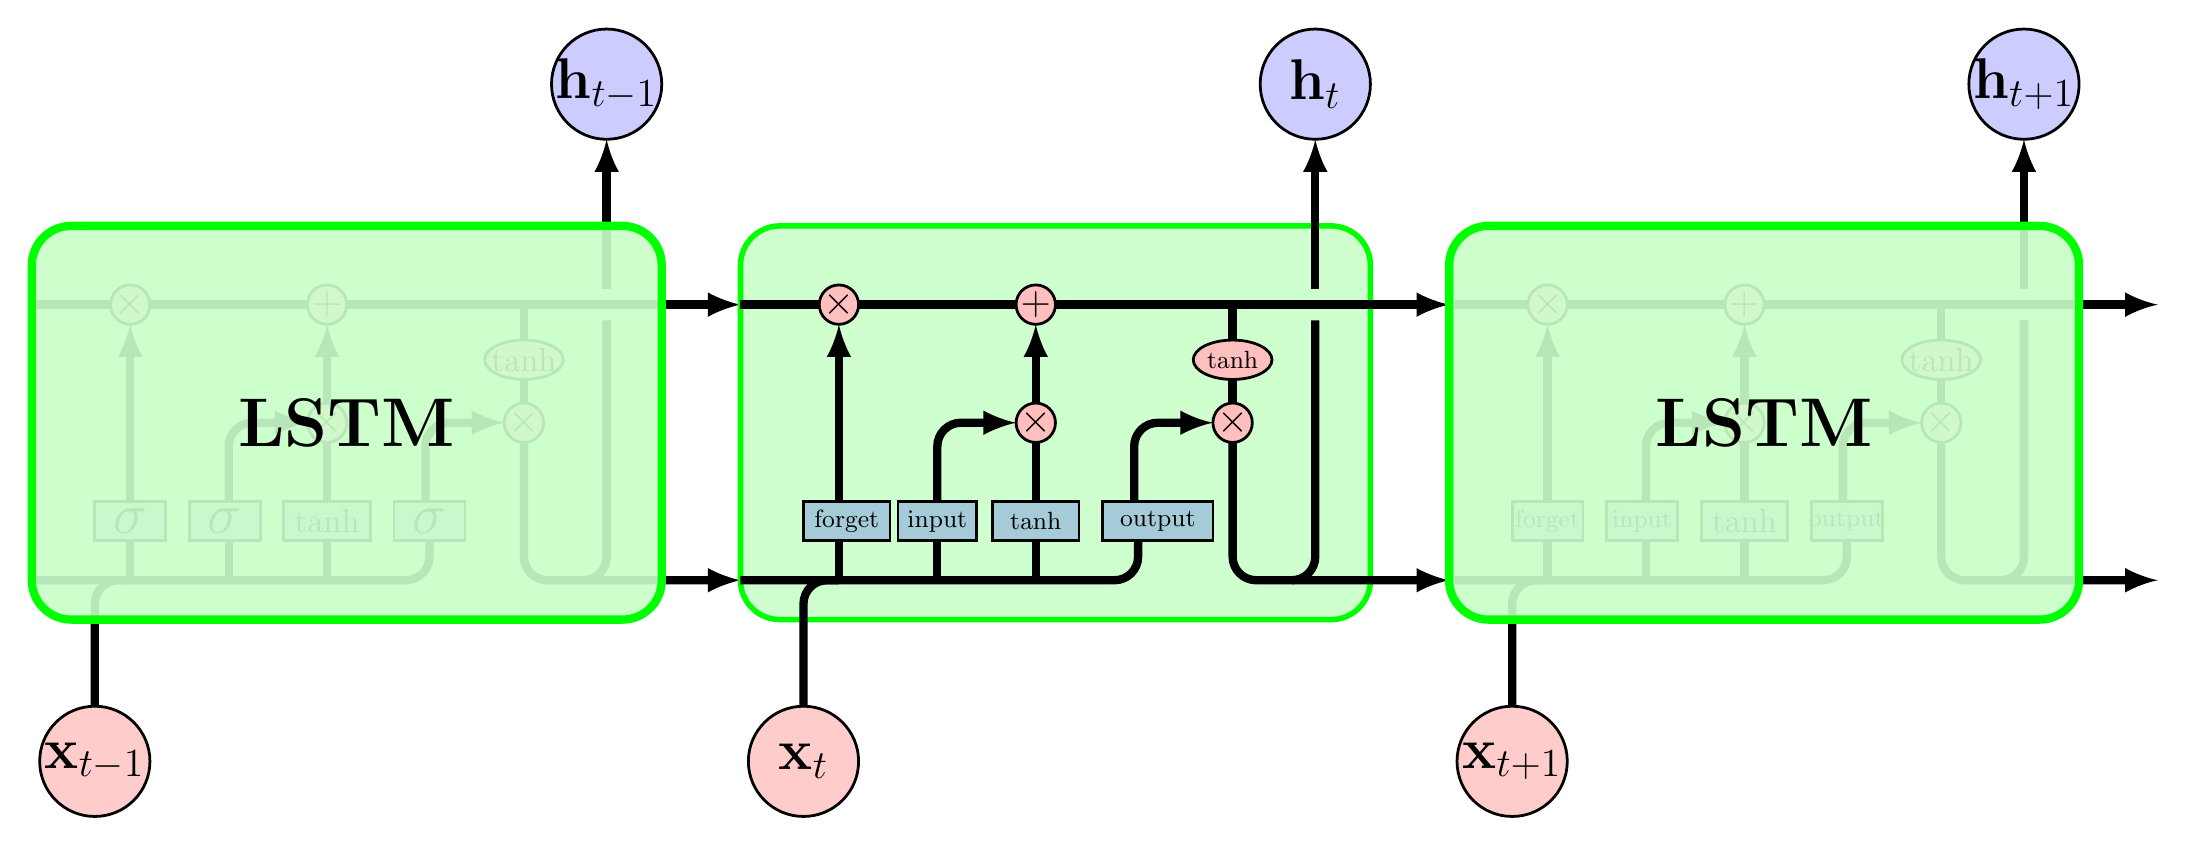
\begin{tikzpicture}
        \coordinate (O) at (0, 0);
        
        \def\offset{0}
        % input
        \filldraw[fill = red,fill opacity=0.2,draw=black,line width=1pt] (-1.2+\offset,0.7) circle (0.7) node[fill opacity=1]{\huge $\mathbf{x}_{t-1}$};
        
        %LSTM
        \filldraw[fill={rgb,255:red,204; green,255; blue,204},fill opacity=0.95,draw=green,line width=2pt,rounded corners=0.5cm] (-2+\offset,2.5) rectangle (6+\offset,7.5); % background
        \filldraw[fill=blue,fill opacity=0.2,draw=black,line width=1pt] (-1.2+\offset,3.5) rectangle (-0.3+\offset,4)node[pos=.5,fill opacity=1]{\huge $\sigma$};
        
        \filldraw[fill=blue,fill opacity=0.2,draw=black,line width=1pt] (0+\offset,3.5) rectangle (0.9+\offset,4)node[pos=.5,fill opacity=1]{\huge $\sigma$};
        
        \filldraw[fill=blue,fill opacity=0.2,draw=black,line width=1pt] (1.2+\offset,3.5) rectangle (2.3+\offset,4)node[pos=.5,fill opacity=1]{\large tanh};
        
        \filldraw[fill=blue,fill opacity=0.2,draw=black,line width=1pt] (2.6+\offset,3.5) rectangle (3.5+\offset,4)node[pos=.5,fill opacity=1]{\huge $\sigma$};
        
        \filldraw[fill=pink,fill opacity=1,draw=black,line width=1pt] (-0.75+\offset,6.5) circle (0.25)node[fill opacity=1]{\Large $\times$};
        
        \filldraw[fill=pink,fill opacity=1,draw=black,line width=1pt] (1.75+\offset,5) circle (0.25)node[fill opacity=1]{\Large $\times$};
        
        \filldraw[fill=pink,fill opacity=1,draw=black,line width=1pt] (4.25+\offset,5) circle (0.25)node[fill opacity=1]{\Large $\times$};
        
        \filldraw[fill=pink,fill opacity=1,draw=black,line width=1pt] (1.75+\offset,6.5) circle (0.25)node[fill opacity=1]{\Large $+$};
        
        \filldraw[fill=pink,fill opacity=1,draw=black,line width=1pt]  (4.25+\offset,5.8) ellipse (0.5cm and 0.25 cm) node[fill opacity=1]{\large tanh};
        
        \draw[ultra thick,black,rounded corners=0.3cm,line width=3pt] (-1.2+\offset,1.4)-- (-1.2+\offset,3)-- (-0.75+\offset,3);
        \draw[ultra thick,black,rounded corners=0.3cm,line width=3pt] (-2+\offset,3)-- (3.05+\offset,3)-- (3.05+\offset,3.5);
        \draw[ultra thick,black,line width=3pt] (-0.75+\offset,3)-- (-0.75+\offset,3.5);
        \draw[-latex,black,line width=3pt] (-0.75+\offset,4)-- (-0.75+\offset,6.25);
        
        \draw[ultra thick,black,line width=3pt] (0.5+\offset,3)-- (0.5+\offset,3.5);
        \draw[-latex,black,rounded corners=0.3cm,line width=3pt] (0.5+\offset,4)-- (0.5+\offset,5)-- (1.5+\offset,5);
        
        \draw[ultra thick,black,line width=3pt] (1.75+\offset,3)-- (1.75+\offset,3.5);
        \draw[ultra thick,black,line width=3pt] (1.75+\offset,4)-- (1.75+\offset,4.75);
        \draw[-latex,black,rounded corners=0.3cm,line width=3pt] (1.75+\offset,5.25)-- (1.75+\offset,6.25);
        
        \draw[ultra thick,black,line width=3pt] (-2+\offset,6.5)-- (-1+\offset,6.5);
        \draw[ultra thick,black,line width=3pt] (-0.5+\offset,6.5)-- (1.5+\offset,6.5);
        \draw[-latex,black,line width=3pt] (2+\offset,6.5)-- (7+\offset,6.5);
        
        \draw[-latex,black,rounded corners=0.3cm,line width=3pt] (3+\offset,4)-- (3+\offset,5)-- (4+\offset,5);
        
        \draw[ultra thick,black,line width=3pt] (4.25+\offset,6.5)-- (4.25+\offset,6.05);
        \draw[ultra thick,black,line width=3pt] (4.25+\offset,5.55)-- (4.25+\offset,5.25);
        \draw[-latex,black,rounded corners=0.3cm,line width=3pt] (4.25+\offset,4.75)-- (4.25+\offset,3)-- (7+\offset,3);
        \draw[ultra thick,black,rounded corners=0.3cm,line width=3pt] (5+\offset,3)-- (5.3+\offset,3) -- (5.3+\offset,6.3);
        \draw[-latex,black,line width=3pt] (5.3+\offset,6.7)-- (5.3+\offset,8.6);
        
        \filldraw[fill = blue,fill opacity=0.2,draw=black,line width=1pt] (5.3+\offset,9.3) circle (0.7)node[fill opacity=1]{\huge $\mathbf{h}_{t-1}$};
        
        \filldraw[fill={rgb,255:red,204; green,255; blue,204},fill opacity=0.9,draw=green,line width=3pt,rounded corners=0.5cm] (-2+\offset,2.5) rectangle (6+\offset,7.5)node[pos=.5,fill opacity=1]{\Huge \textbf{LSTM}};
        
        
        \def\offset{9}
        % input
        \filldraw[fill = red,fill opacity=0.2,draw=black,line width=1pt] (-1.2+\offset,0.7) circle (0.7) node[fill opacity=1]{\huge $\mathbf{x}_{t}$};
        
        %LSTM
        \filldraw[fill={rgb,255:red,204; green,255; blue,204},fill opacity=0.95,draw=green,line width=2pt,rounded corners=0.5cm] (-2+\offset,2.5) rectangle (6+\offset,7.5); % background
        \filldraw[fill=blue,fill opacity=0.2,draw=black,line width=1pt] (-1.2+\offset,3.5) rectangle (-0.1+\offset,4)node[pos=.5,fill opacity=1]{\small forget};
        
        \filldraw[fill=blue,fill opacity=0.2,draw=black,line width=1pt] (0+\offset,3.5) rectangle (1+\offset,4)node[pos=.5,fill opacity=1]{\small input};
        
        \filldraw[fill=blue,fill opacity=0.2,draw=black,line width=1pt] (1.2+\offset,3.5) rectangle (2.3+\offset,4)node[pos=.5,fill opacity=1]{\small tanh};
        
        \filldraw[fill=blue,fill opacity=0.2,draw=black,line width=1pt] (2.6+\offset,3.5) rectangle (4+\offset,4)node[pos=.5,fill opacity=1]{\small output };
        
        \filldraw[fill=pink,fill opacity=1,draw=black,line width=1pt] (-0.75+\offset,6.5) circle (0.25)node[fill opacity=1]{\Large $\times$};
        
        \filldraw[fill=pink,fill opacity=1,draw=black,line width=1pt] (1.75+\offset,5) circle (0.25)node[fill opacity=1]{\Large $\times$};
        
        \filldraw[fill=pink,fill opacity=1,draw=black,line width=1pt] (4.25+\offset,5) circle (0.25)node[fill opacity=1]{\Large $\times$};
        
        \filldraw[fill=pink,fill opacity=1,draw=black,line width=1pt] (1.75+\offset,6.5) circle (0.25)node[fill opacity=1]{\Large $+$};
        
        \filldraw[fill=pink,fill opacity=1,draw=black,line width=1pt]  (4.25+\offset,5.8) ellipse (0.5cm and 0.25 cm) node[fill opacity=1]{\small tanh};
        
        \draw[ultra thick,black,rounded corners=0.3cm,line width=3pt] (-1.2+\offset,1.4)-- (-1.2+\offset,3)-- (-0.75+\offset,3);
        \draw[ultra thick,black,rounded corners=0.3cm,line width=3pt] (-2+\offset,3)-- (3.05+\offset,3)-- (3.05+\offset,3.5);
        \draw[ultra thick,black,line width=3pt] (-0.75+\offset,3)-- (-0.75+\offset,3.5);
        \draw[-latex,black,line width=3pt] (-0.75+\offset,4)-- (-0.75+\offset,6.25);
        
        \draw[ultra thick,black,line width=3pt] (0.5+\offset,3)-- (0.5+\offset,3.5);
        \draw[-latex,black,rounded corners=0.3cm,line width=3pt] (0.5+\offset,4)-- (0.5+\offset,5)-- (1.5+\offset,5);
        
        \draw[ultra thick,black,line width=3pt] (1.75+\offset,3)-- (1.75+\offset,3.5);
        \draw[ultra thick,black,line width=3pt] (1.75+\offset,4)-- (1.75+\offset,4.75);
        \draw[-latex,black,rounded corners=0.3cm,line width=3pt] (1.75+\offset,5.25)-- (1.75+\offset,6.25);
        
        \draw[ultra thick,black,line width=3pt] (-2+\offset,6.5)-- (-1+\offset,6.5);
        \draw[ultra thick,black,line width=3pt] (-0.5+\offset,6.5)-- (1.5+\offset,6.5);
        \draw[-latex,black,line width=3pt] (2+\offset,6.5)-- (7+\offset,6.5);
        
        \draw[-latex,black,rounded corners=0.3cm,line width=3pt] (3+\offset,4)-- (3+\offset,5)-- (4+\offset,5);
        
        \draw[ultra thick,black,line width=3pt] (4.25+\offset,6.5)-- (4.25+\offset,6.05);
        \draw[ultra thick,black,line width=3pt] (4.25+\offset,5.55)-- (4.25+\offset,5.25);
        \draw[-latex,black,rounded corners=0.3cm,line width=3pt] (4.25+\offset,4.75)-- (4.25+\offset,3)-- (7+\offset,3);
        \draw[ultra thick,black,rounded corners=0.3cm,line width=3pt] (5+\offset,3)-- (5.3+\offset,3) -- (5.3+\offset,6.3);
        \draw[-latex,black,line width=3pt] (5.3+\offset,6.7)-- (5.3+\offset,8.6);
        
        \filldraw[fill = blue,fill opacity=0.2,draw=black,line width=1pt] (5.3+\offset,9.3) circle (0.7)node[fill opacity=1]{\huge $\mathbf{h}_{t}$};
        
        %\filldraw[fill={rgb,255:red,204; green,255; blue,204},fill opacity=0.9,draw=green,line width=3pt,rounded corners=0.5cm] (-2+\offset,2.5) rectangle (6+\offset,7.5)node[pos=.5,fill opacity=1]{\Huge \textbf{LSTM}};
        
        
        \def\offset{18}
        % input
        \filldraw[fill = red,fill opacity=0.2,draw=black,line width=1pt] (-1.2+\offset,0.7) circle (0.7) node[fill opacity=1]{\huge $\mathbf{x}_{t+1}$};
        
        %LSTM
        \filldraw[fill={rgb,255:red,204; green,255; blue,204},fill opacity=0.95,draw=green,line width=2pt,rounded corners=0.5cm] (-2+\offset,2.5) rectangle (6+\offset,7.5); % background
        \filldraw[fill=blue,fill opacity=0.2,draw=black,line width=1pt] (-1.2+\offset,3.5) rectangle (-0.3+\offset,4)node[pos=.5,fill opacity=1]{\small forget};
        
        \filldraw[fill=blue,fill opacity=0.2,draw=black,line width=1pt] (0+\offset,3.5) rectangle (0.9+\offset,4)node[pos=.5,fill opacity=1]{\small input};
        
        \filldraw[fill=blue,fill opacity=0.2,draw=black,line width=1pt] (1.2+\offset,3.5) rectangle (2.3+\offset,4)node[pos=.5,fill opacity=1]{\large tanh};
        
        \filldraw[fill=blue,fill opacity=0.2,draw=black,line width=1pt] (2.6+\offset,3.5) rectangle (3.5+\offset,4)node[pos=.5,fill opacity=1]{\small output};
        
        \filldraw[fill=pink,fill opacity=1,draw=black,line width=1pt] (-0.75+\offset,6.5) circle (0.25)node[fill opacity=1]{\Large $\times$};
        
        \filldraw[fill=pink,fill opacity=1,draw=black,line width=1pt] (1.75+\offset,5) circle (0.25)node[fill opacity=1]{\Large $\times$};
        
        \filldraw[fill=pink,fill opacity=1,draw=black,line width=1pt] (4.25+\offset,5) circle (0.25)node[fill opacity=1]{\Large $\times$};
        
        \filldraw[fill=pink,fill opacity=1,draw=black,line width=1pt] (1.75+\offset,6.5) circle (0.25)node[fill opacity=1]{\Large $+$};
        
        \filldraw[fill=pink,fill opacity=1,draw=black,line width=1pt]  (4.25+\offset,5.8) ellipse (0.5cm and 0.25 cm) node[fill opacity=1]{\large tanh};
        
        \draw[ultra thick,black,rounded corners=0.3cm,line width=3pt] (-1.2+\offset,1.4)-- (-1.2+\offset,3)-- (-0.75+\offset,3);
        \draw[ultra thick,black,rounded corners=0.3cm,line width=3pt] (-2+\offset,3)-- (3.05+\offset,3)-- (3.05+\offset,3.5);
        \draw[ultra thick,black,line width=3pt] (-0.75+\offset,3)-- (-0.75+\offset,3.5);
        \draw[-latex,black,line width=3pt] (-0.75+\offset,4)-- (-0.75+\offset,6.25);
        
        \draw[ultra thick,black,line width=3pt] (0.5+\offset,3)-- (0.5+\offset,3.5);
        \draw[-latex,black,rounded corners=0.3cm,line width=3pt] (0.5+\offset,4)-- (0.5+\offset,5)-- (1.5+\offset,5);
        
        \draw[ultra thick,black,line width=3pt] (1.75+\offset,3)-- (1.75+\offset,3.5);
        \draw[ultra thick,black,line width=3pt] (1.75+\offset,4)-- (1.75+\offset,4.75);
        \draw[-latex,black,rounded corners=0.3cm,line width=3pt] (1.75+\offset,5.25)-- (1.75+\offset,6.25);
        
        \draw[ultra thick,black,line width=3pt] (-2+\offset,6.5)-- (-1+\offset,6.5);
        \draw[ultra thick,black,line width=3pt] (-0.5+\offset,6.5)-- (1.5+\offset,6.5);
        \draw[-latex,black,line width=3pt] (2+\offset,6.5)-- (7+\offset,6.5);
        
        \draw[-latex,black,rounded corners=0.3cm,line width=3pt] (3+\offset,4)-- (3+\offset,5)-- (4+\offset,5);
        
        \draw[ultra thick,black,line width=3pt] (4.25+\offset,6.5)-- (4.25+\offset,6.05);
        \draw[ultra thick,black,line width=3pt] (4.25+\offset,5.55)-- (4.25+\offset,5.25);
        \draw[-latex,black,rounded corners=0.3cm,line width=3pt] (4.25+\offset,4.75)-- (4.25+\offset,3)-- (7+\offset,3);
        \draw[ultra thick,black,rounded corners=0.3cm,line width=3pt] (5+\offset,3)-- (5.3+\offset,3) -- (5.3+\offset,6.3);
        \draw[-latex,black,line width=3pt] (5.3+\offset,6.7)-- (5.3+\offset,8.6);
        
        \filldraw[fill = blue,fill opacity=0.2,draw=black,line width=1pt] (5.3+\offset,9.3) circle (0.7)node[fill opacity=1]{\huge $\mathbf{h}_{t+1}$};
        
        \filldraw[fill={rgb,255:red,204; green,255; blue,204},fill opacity=0.9,draw=green,line width=3pt,rounded corners=0.5cm] (-2+\offset,2.5) rectangle (6+\offset,7.5)node[pos=.5,fill opacity=1]{\Huge \textbf{LSTM}};
        \end{tikzpicture}
         }
\caption{Structure of LSTM cells}
\label{fig:lstm_cell}
\end{figure}

Forget Gate: The sigmoid function generates a value between 0 and 1 in the forget gate, which is the first step, to indicate how much knowledge of the prior hidden state and the present input it should keep. Input Gate:The following action has two components. The input gate chooses the new data to be stored in the memory cell first. A tanh layer then creates a vector of new candidate values that will be added to the state. Output gate : Applying the sigmoid function to the prior hidden state and current input and multiplying it by the tanh function applied to the new memory cell will provide values between -1 and 1 for the memory cell's output. The equations for the forget, input and output gates in LSTM are presented in \ref{Eq:forget_lstm}, \ref{Eq:output_lstm}:

\begin{equation}\label{Eq:forget_lstm}
    f_t\ =\sigma (w_f[h^{t-1},x^t]+b_f)
\end{equation}

\begin{equation}\label{Eq:input_lstm}
    i_t\ =\ \sigma\ (w_i[h^{t-1},x^t]+b_i)
\end{equation}

\begin{equation}\label{Eq:output_lstm}
    o_t\ =\sigma (w_o[h^{t-1},x^t]+b_o)
\end{equation}

Where :
$I_t$ = represents the input gate.\\
$F_t$ = represents the forget gate.\\
$O_t$ = represents the output gate. \\
$\sigma$ = represents sigmoid function.\\
$W_x$= weight for the respective gate (x) neurons.\\
$H^{t-1}$ = output of the previous lstm block (at timestamp t-1)\\
$X^t$ =input at current timestamp. \\
%$B_x$ = biases for the respective gates (X)
	
The equations for the cell state, candidate cell state and the final output:
\begin{equation}
   \tilde{C}^t = tanh (wc [ht-1,xt]+ bc ) 
\end{equation}

\begin{equation}
    C^t\ =\ F_t\ \times C^{t-1}+I_t\times \tilde{C}^t
\end{equation}

\begin{equation}
    H_t\ =\ o_t\times tanh(C^t)
\end{equation}
Where :
$Ct$ = cell state (memory) at timestamp (t).\\
$\tilde{C}^t$ = represents candidate for cell state at timestamp (t).\\

The gate units of the bidirectional LSTM are identical to the LSTM. Bi-LSTM is a combination of a forward LSTM and a backward LSTM, that means, one time step of data is input simultaneously in both forward and reverse directions. Although Bi-LSTM needs to train more generations to converge to stability, it also has higher precision because it gets more input information. So we chose the Bi-LSTM as the prediction model.

\section{Experiments}
% symbolic regression generations and population

%neural networks and hyperparamters tuning 
In this section, we will validate and evaluate the proposed models using the electrical submersible pumps data set that we have explored earlier this chapter. 


When we usually use neural networks to build models, the size of the network layer
and the number of neurons are not strictly defined. We determined the parameters of each layer of the model through multiple experimental adjustments. Specifically, we set up two layers of convolution layers, the filters size of each convolution layer was set to 3, and the Relu function was used. Two layers of Bi-LSTM, the previous layer of neurons was set to 30, and the latter layer was set to 24 which is determined by the output dimension of the model. In addition, all models are supervised trained using Adam algorithm that optimizes a predetermined objective function, to obtain model

\section{Summary}
In order to monitor and improve the production processes, it is crucial to estimate multiphase flowrates correctly. In typical field operations, the estimation of well flowrates is done by directing stream from a specific well into a test separator where it is split into oil, gas and water. This traditional method has a disadvantage of not being able to identify production trends. Another technology is invented to estimate production rates by measuring one physical property of the stream and relate it to different fluids rates. It is called multiphase flow metes (MPFMs). The aforementioned methods have high capital and operating expenses for such meter’s maintenance. 

A solution involving machine learning and physics based transient modeling is an alternative to the usage of MPFMs and production testing. It is called virtual flow meters (VFM). It arises as an attractive research area in oil and gas industry. It depends on either analytical or data driven models for real time calculations of production phases.

In this chapter, a new data driven model was introduced to calculate the multiphase flow rate using sensors measurements of the electrical submersible pumps. In addition, a framework is introduced for detailed exploratory data analysis and calibrating the proposed model to account for production conditions. Then, feature prioritization experiments are conducted to identify the most dominant parameters that affects rates prediction. Finally, the mean absolute error, mean squared error, and r squared are used to compare the models. 

In this work we have used a real time data set from ESP assisted wells. Our method encompassed the implementation of symbolic regression, and deep learning. Convolutional neural network pipeline with long short term memory algorithm (LSTM) are used for real time prediction of liquid rate and water cut based on sensors’ data.  



\chapter{Predictive maintenance for electrical submersible pumps}

\section{Introduction}
As any pumping artificial lift method, \ac{ESP}s exhibit failures. The maintenance of \ac{ESP}s expends a lot of resources and manpower and is usually triggered and accompanied by the reactive process monitoring of multivariate sensor data.

In general, this chapter work focusing on the usage of machine learning to understanding an equipment status so as to facilitate predictive maintenance and to avoid operation downtime. ESPs are installed in many producing wells that are subject to harsh environments and need to pump complex fluid mixtures that on their turn undergo changes in composition, pressure and temperature over time. For assuring a reliable fluid delivery, on time interventions are required in case of upcoming problems. Hence, strong efforts are undertaken in the area of “digital oil field”, that focus on deploying machine learning and data-driven models in the area of predictive pump maintenance of electrical submersible pumps.

In this chapter, we introduce a contribution to the area of efficiency increase by reducing the time required to dismantle the system, inspect it and perform failure analysis. The objective is achieved by applying the \ac{PCA} as a dimentionality reduction technique then its output is pipelined with a model trained using\ac{XGBoosting} algorithm for future prediction of the system pre-workver events.

The proposed model is able to identify deeper functional relationships and longer-term trends inferred from historical data. The novel workflow with the predictive model can provide alarms within seven days before the actual failure event. 

\section{Data gathering and Pre-Processing}

Time series data are collected from sensors on \ac{ESP} wells. The reported measurements are \ac{FRQ}, \ac{PDP}, \ac{PIP}, \ac{WHP}, \ac{WHT}, \ac{MT}, \ac{CHP} and \ac{Current}. They have different frequencies. Also well status sheets for the same wells at the same time periods are gathered in daily frequency. These data come from a field that has a polymer flooding project. Based on the status sheets, pumps exhibits two main categories of problems. Those are \ac{MDHF} and \ac{EDHF} therefore both are laying under electrical pump failures. 

Electric Failures of the downhole facilities, both \ac{MDHF} and \ac{EDHF}, are failures of any of the electrical components in the ESP assembly including the electric cable, the motor electrical components such as the stator, and the downhole sensor. Failures associated with the electric cables are mainly caused by cable insulation due to corrosion, material failure, cable failure due to overload. While electrical failures associated with the motor are usually a resultant of the stator failure. The stator has been reported to fail due to overheating due to temperature. As the motor is the hottest point in the well, this appears to worsen polymer deposition on the motor body. This in turn reduces heat dissipation leading to increasing motor winding temperature, which in turn make the deposition worse and eventual ramp down of ESP frequency when maximum motor temperatures are reached. Likewise, the high temperatures around the motor aids on the precipitation of solid polymer in fluids flowing past the motor and are the source of polymer plugging in the pump inlet.     

The workflow in predictive modelling starts with the data cleaning process. On one hand It is important to eliminate nonphysical values (e.g., negative or enormous pressure values), remove further outliers and align units. On the other hand, it is a critical step for handling noise data while maintaining the realistic anomalies that may identify downhole problems of the pumps. 

After visual inspection of the data, a pipeline of a pre-processing strategy is created. Firstly, it starts by resampling the data using a moving median in one-hour steps. Fig \ref{fig:boxplot_before_outlier} shows the boxplot of the data after re-sampling and before outliers removal. It is obvious that some measurements include unreasonable measurements. For example, Well head temperature reaches 18500 $^{\circ}$F which is obviously error measurement. Therefore, the second step is removing outliers. It includes first removing measurements where oil production is zero then outlier removal by limits.

\begin{figure}
    \centering
    
\includegraphics[width=\textwidth]{figures/predictive_maintenance/Fig 2-updates.png}
    \caption{Box-plot before outlier removal}
    \label{fig:boxplot_before_outlier}
\end{figure}

Outlier removal by limits depends mainly on quartiles therefore we used boxplots. They summarizes sample data using 25th, 50th, and 75th quartiles. The mid-spread or middle 50th, or technically H-spread, is a measure of statistical dispersion, being equal to the difference between 75th and 25th percentiles. It is called the interquartile range (IQR). IQR is somewhat similar to Z-score in terms of finding the distribution of data and then keeping some threshold to identify the outlier. To define the outlier base value is defined above and below datasets normal range namely Upper and Lower bounds. the upper and the lower bound are calculated according to equation \ref{Eq:upper_boundary} and \ref{Eq:lower_boundary}.

\begin{equation}\label{Eq:lower_boundary}
   upper = Q3 +1.5 * IQR  
\end{equation}
\begin{equation}\label{Eq:upper_boundary}
   lower = Q1 – 1.5 * IQR 
\end{equation}

Afterwards, a standard scaler is employed (subtracting mean from each point and dividing by the variance) transforming the mean value to zero and scaling the data to unit variance. Finally, the moving difference is applied on all sensors measurements. Fig. \ref{fig:boxplot_after_outlier} shows the box plot after outliers removal. Fig. \ref{fig:boxplot_after_normalization} shows the box plot after normalization.   

\begin{figure}
    \centering
    
\includegraphics[width=\textwidth]{figures/predictive_maintenance/Fig 3-Updated.png}
    \caption{Box-plot after outlier removal}
    \label{fig:boxplot_after_outlier}
\end{figure}

\begin{figure}
    \centering
    
\includegraphics[width=\textwidth]{figures/predictive_maintenance/Fig 4-updated.png}
    \caption{Box-plot after outlier normalization}
    \label{fig:boxplot_after_normalization}
\end{figure}

Table \ref{tab:esp_eda} describes the main signals after outliers and zero production points are removed without standardization. Table \ref{tab:class_esp} shows the number of available data points after mapping the sensor data. These data points are classified, based on workover sheets, into “Normal data”, “Pre-workover”, and “Workover”. Pre-workover data are data points that are reported seven days before the workover day. Workover events are the data points made available on workover day.  

\begin{table}[]
\center
\resizebox{\textwidth}{!}{%
\begin{tabular}{l|S[round-mode = places]|S[round-mode = places]|S[round-mode = places]|S[round-mode = places]|S[round-mode = places]|S[round-mode = places]|S[round-mode = places]|S[round-mode = places]|}
\cline{2-9}
                          & \ac{FRQ}[Hz] & \ac{PDP}[Psi] & \ac{PIP}[Psi] & \ac{WHP} [Psi] & \ac{WHT}[$^\circ$F] & MT[$^\circ$F]  & \ac{CHP}[Psi] & \ac{Current} [A] \\ \hline
\multicolumn{1}{|l|}{mean} & 52.6806238 & 1522.96643 & 855.891601 & 642.207855 & 62.3826216 & 137.11823  & 922.12718  & 349.645672 \\ \hline
\multicolumn{1}{|l|}{std}  & 4.29171119 & 187.461024 & 211.079864 & 608.613357 & 11.487392  & 32.397163  & 1883.03087 & 86.9083859 \\ \hline
\multicolumn{1}{|l|}{min} & 35       & 1086.5156 & 610.456   & 194.059   & 60.545  & 120.626 & 0         & 101.5963    \\ \hline
\multicolumn{1}{|l|}{25\%} & 49.702205  & 1506.13425 & 660.900075 & 213.385671 & 63.231987  & 122.2008   & 91.5382681 & 317.009525 \\ \hline
\multicolumn{1}{|l|}{50\%} & 52.76629   & 1543.801   & 721.8032   & 243.580588 & 65.9961325 & 154.192608 & 261.378201 & 354.0059   \\ \hline
\multicolumn{1}{|l|}{75\%} & 56.58294   & 1595.04975 & 778.89995  & 547.3371   & 67.6575825 & 160.6      & 405.28695  & 394.737969 \\ \hline
\multicolumn{1}{|l|}{max}  & 64.964555  & 1893.238   & 1578.28725 & 845.8625   & 122.843    & 169.3002   & 986.7425   & 598.211    \\ \hline
\end{tabular}%
}
\caption{Data Exploration}
\label{tab:esp_eda}
\end{table}

\begin{table}[]
\center
\begin{tabular}{|l|l|}
\hline
Condition    & Reported Data Points \\ \hline
Normal       & 339,089              \\ \hline
Pre-Workover & 1728                 \\ \hline
Workover     & 288                  \\ \hline
\end{tabular}%
\caption{Data Points Classification}
\label{tab:class_esp}
\end{table}

\section{\ac{PCA} Application }
\ac{PCA} is defined as an unsupervised dimensionality reduction technique. It reduces large dimensionality data sets into lower dimensions called principle components. This happens while preserving as much information as possible. It makes use of the interdependence of original data to build a \ac{PCA} model. This results in reducing the dimension of production parameters by making the most of the linear combinations and by generating a new Principal Component space (PCs)

\subsection{\ac{PCA} Calculations}
The process of obtaining a \ac{PCA} model from a raw dataset is divided into four steps as follows:
Firstly, the covariance matrix $\sum$ of the whole dataset is computed. It is important to see whether there is a relationship between contributing features. Equation \ref{Eq:cov_matrix} is used to find the covariance between each pair of dataset columns. 

\begin{equation}\label{Eq:cov_matrix}
    \sum =\ \frac{1}{n-1}\sum_{i=1}^{n}{(X_{ij}-\widetilde{x_j})(X_{ik}-\widetilde{x_k})}
\end{equation}
\nomenclature{$\sum$}{Covariance}
\nomenclature{$a$}{sldldsm sldm l}

The second step is to calculate eigenvectors and corresponding eigenvalues. Let A be the covariance matrix that has been computed in the first step, $\nu$ a vector and $\lambda$ a scalar that satisfies $A\nu=\lambda\nu$, then $\lambda$ is the eigenvalue corresponding to eigenvector $\nu$ of A. This step is considered the calculation of the principal components of the data.

The third step is determining the number of principal components. The eigenvectors only define the directions of the new axis while the eigenvalues represent the variance of the data along the new feature axes. Therefore, we sort the eigenvectors based on the eigenvalues. Hence, a threshold is chosen on the eigenvalues and cut off is made on the eigenvectors to select the most informative lower dimensional subspace. In other words, Lower variance dimensions are omitted. This is because they possess the least information about the data’s distribution.

The Fourth step consists of transforming the samples into the new subspace. In this last step, the lower dimensional subspace $W$ is selected. In the current step, the dataset samples are transformed into this new subspace via the equation $Y = W^ \prime. X$ where $W^\prime$ is the transpose of the matrix W. In the following, two principal components are computed and the data points are reoriented onto the new subspace. Fig. \ref{fig:pca} shows the simple geometric meaning of \ac{PCA}.

\begin{figure}
    \centering
    
\includegraphics[keepaspectratio, width=\textwidth]{figures/predictive_maintenance/Fig 5.png}
    \caption{Geometric meaning of \ac{PCA}}
    \label{fig:pca}
\end{figure}

\subsection{Application of \ac{PCA} in the Electrical Submersible Pumps}
In ESP systems, sensor data are generally highly correlated, e.g., wellhead pressure is directly proportional to discharge and intake pressures. However, when a downhole problem occurs or is about to occur, anomalous data can be identified because it breaks certain rules in the input signals and their relative changes, i.e., if there is a tubing leak, the annulus discharge pressure decreases while intake pressure and annulus pressure increases, etc. 
Principal Component Analysis then suits the engineers’ purpose to create an anomaly detection system. This is mainly because it makes use of the interdependence of original data to build a model. The primary goal of this step is to create clusters out of the data.
As discussed earlier, the selection of the principal components is made based on the maximum variance criterion. The highest variance is captured in the first principal component while the next highest variance is captured in the second principal component, where information from the first principal component has already been removed. In a similar manner, consecutive principal components (3rd, 4th, ……, Kth) can be constructed to evaluate the original system. 
The PCA model finds the kth principal component to construct the PCs, where most of the information belonging to the initial system is contained. The kth principal component is represented in equation \ref{Eq:pcs} below where PC1 is given as an example.

\begin{equation}\label{Eq:pcs}
\begin{split}
    {PC}_k=a_{1k}\ast P_{intake\ pressure}+\ a_{2k}
    \ast P_{discarge\ pressure}+\ a_{3k}P_{Motor\ temperature}+\ldots \\
+a_{pk}P_{intake\ pressure\ moving\ difference}+..
\end{split}
\end{equation}

Figure \ref{fig:pca_esp} shows the projection of ESP well sensor data on the principal components. The developed model is used also to evaluate near failure conditions. The problematic days and seven days before workover, sensor data clearly show specific failure patterns in line with the reported \ac{MDHF} and \ac{EDHF}.

\begin{figure}
    \centering
    
\includegraphics[keepaspectratio, width=\textwidth]{figures/predictive_maintenance/Fig 6.png}
    \caption{"Principle component analysis of ESP wells"}
    \label{fig:pca_esp}
\end{figure}

The goal of the \ac{PCA} is to come up with optimal weights from each sensor measurement. That means capturing as much information as possible from the input signals, based on the correlations among those variables. the loadings are the correlations between the variables and the component. We compute the weights in the weighted average from these loadings. To compute the Loading matrix, namely the correlations between the original variable and the principal components, the cross-covariance matrix is needed to be computed from equation \ref{Eq:cross_cov}.

\begin{equation}\label{Eq:cross_cov}
    Cov\left(X,\ Y\right)=V\sqrt E
\end{equation}

 Where: X is the original variables,
 	Y is the principal components,
 	V is the principal axes
E are its eigenvalues.
Table 4 represent the load factor for each input parameter in the relevant principle component till the 8th principle component. However, we mostly interested in parameters loading factors on the first and second principle component because they explain approximately 0.6 of the data variance as shown previously in figure 7. Large loadings (positive or negative) indicate that a particular variable has a strong relationship to a particular principal component. The sign of a loading indicates whether a variable and a principal component are positively or negatively correlated42. Hence, the most parameters correlated parameters with the first principle component are pump frequency, casing head pressure, current, motor temperature and well head temperature. 

% Please add the following required packages to your document preamble:
% \usepackage{graphicx}
\begin{table}[]
\resizebox{\textwidth}{!}{%
\begin{tabular}{|l|l|l|l|l|l|l|l|l|}
\hline
              & PC1   & PC2   & PC3   & PC4   & PC5   & PC6   & PC7   & PC8   \\ \hline
FRQ           & -0.90 & -0.05 & 0.06  & 0.05  & -0.05 & -0.26 & 0.05  & 0.01  \\ \hline
PDP           & -0.54 & -0.14 & -0.70 & 0.32  & -0.07 & -0.08 & 0.04  & 0.05  \\ \hline
PIP           & 0.03  & -0.17 & -0.47 & 0.14  & -0.05 & 0.81  & -0.18 & -0.04 \\ \hline
WHP           & 0.10  & -0.02 & -0.79 & 0.37  & -0.01 & -0.15 & 0.23  & -0.28 \\ \hline
WHT           & -0.63 & 0.00  & 0.35  & -0.30 & 0.18  & 0.22  & 0.12  & -0.32 \\ \hline
MT            & -0.79 & -0.12 & -0.07 & 0.04  & -0.12 & 0.25  & -0.16 & 0.22  \\ \hline
CHP           & -0.85 & -0.15 & -0.07 & 0.15  & -0.03 & -0.27 & 0.07  & 0.12  \\ \hline
CURRENT       & -0.84 & -0.10 & 0.21  & -0.17 & 0.07  & 0.21  & -0.06 & -0.19 \\ \hline
diff\_FRQ     & -0.14 & 0.78  & 0.03  & 0.27  & 0.09  & 0.02  & -0.22 & -0.17 \\ \hline
diff\_PDP     & -0.05 & 0.09  & -0.45 & -0.54 & 0.21  & -0.19 & -0.40 & 0.28  \\ \hline
diff\_PIP     & 0.06  & -0.35 & -0.34 & -0.67 & -0.21 & 0.06  & 0.18  & 0.11  \\ \hline
diff\_WHP     & -0.03 & 0.11  & -0.42 & -0.50 & 0.36  & -0.15 & -0.05 & -0.42 \\ \hline
diff\_WHT     & -0.10 & 0.43  & -0.08 & -0.11 & 0.37  & 0.23  & 0.69  & 0.26  \\ \hline
diff\_MT      & -0.15 & 0.84  & -0.10 & -0.10 & -0.34 & 0.03  & -0.03 & -0.03 \\ \hline
diff\_CHP     & 0.03  & -0.29 & 0.03  & 0.30  & 0.85  & 0.01  & -0.14 & 0.11  \\ \hline
diff\_CURRENT & -0.13 & 0.80  & -0.14 & -0.04 & 0.16  & 0.05  & -0.09 & 0.20  \\ \hline
\end{tabular}%
}
\caption{Loading for input parameters}
\label{input_loading_pca}
\end{table}


\section{\ac{XGBoosting} Application}
\ac{XGBoosting} is a tree-based ensemble model. Ensemble learning is a systematic solution that combines the predictive abilities of multiple models, eventually resulting in a single model. This single model provides the aggregated output of several models that, on their turn, only perform slightly better than random guessing. Therefore, Extreme Gradient Boosting (XGBoost) is an ensemble set of predictors, with a unified objective of predicting the same target variable. A final prediction is performed through the combination of these set of predictors.	
\subsection{\ac{XGBoosting} Calculations  }
Building an XGBoost model has the following sequence. It starts with a single root (contains all the training samples). Then, an iteration is performed over all features and values per feature and subsequently, each possible split loss reduction is evaluated. Equations 6 and 7 represent the objective function (loss function and regularization, respectively) at each iteration that is needed to be minimized.
\begin{equation}
\mathcal{L}^{\left(t\right)}=\ \sum_{i=1}^{n}{l\left(y_i,p_i+\ O_{value}\right)+\frac{1}{2}\lambda}O_{value}^2    
\end{equation}
\begin{equation}
    l\left(y_i,p_i\right)=-\left[y_i\log{\left(p_i\right)+\left(1-y_i\right)\log{\left(1-p_i\right)}}\right]
\end{equation}
Where: \\
$y_i$ is the true value required to be predicted of the i-th instance \\
$p_i$ is the prediction of the i-th instance\\
$\left(y_i,p_i\right)$ The loss function for typical classification problem \\
$O_{value}$ The output of the new tree\\
$\frac{1}{2}\lambda O_{value}^2$ Regularization Term\\

Tianqui stated “XGBoost objective function cannot be optimized using traditional optimization methods in Euclidean space”44. Therefore, in order to be able to transform this objective function to the Euclidean domain, the second-order Taylor approximation is used enabling traditional optimization techniques to be employed. Equation 8 and 9 represent the Taylor approximation of the loss function.

\begin{equation}
    \mathcal{L}^{(t)}\cong[\sum_{i=1}^{n}{l\left(y_i,p_i\right)+g_iO_{value}+\frac{1}{2}h_iO_{value}^2}]+\frac{1}{2}\lambda}O_{value}^2    
\end{equation}

Where: \\ 
$g_i$ is the gradient and calculated by $g_i=\ \frac{\partial}{\partial p_i}l(y_i,\ p_i)$  \\
$h_i$ is the hessian and calculated by $h_i=\ \frac{\partial^2}{\partial p_i^2}l(y_i,\ p_i)$ \\     	 	 	 	
Finally, removing the constant parts, the simplified objective to minimize at step t, results in:
\begin{equation}
    \mathcal{L}^{(t)}=\ \sum_{i=1}^{n}{g_iO_{value}+\frac{1}{2}h_iO_{value}^2+\frac{1}{2}\lambda O_{value}^2}		
\end{equation}

Equations 10 and 11 show how to minimize that function 

\begin{equation}
\frac{d}{dO_{value}}\ \sum_{i=1}^{n}{g_iO_{value}+\frac{1}{2}h_iO_{value}^2}+\frac{1}{2}\lambda O_{value}^2=0    
\end{equation}

\begin{equation}
    O_{value}=\ -\ \frac{\sum_{i=1}^{n}g_i}{\sum_{i}^{n}{h_i+\lambda}}					
\end{equation}

By combining equation 10 with the first and the second derivative of the classification loss function $g_i$ and $h_i$, the similarity equation is derived. The similarity score is calculated as follows in equation 12: 

\begin{equation}
    Similarity\ =\frac{\sum{Residual}_i}{\sum{{Previous\ Probability}_i\ast\ \left(1-{Previous\ Probability}_i\right)+\ \lambda}}\
\end{equation}

The similarity score is calculated for a “leaf” of the “tree”. Various thresholds are used to split the tree into more leaves. The similarity score is calculated for each new leaf followed by calculating the so-called gain as presented in equation 13 below: 

\begin{equation}
    Gain={Left}_{similarity}+{Right}_{similarity}-{Root}_{similarity}	
\end{equation}

Then thresholds continue to be set until higher gain thresholds are reached and the tree keeps growing. There is a minimum number of residuals in each leaf where the tree stops growing. This number is determined by calculating a parameter called cover. It is defined as the denominator of the similarity score minus lambda. During boosting, the operation is performed such that trees are sequentially constructed. Each tree reduces the error of its predecessor and learns from it while simultaneously updating the residual errors. As a result, each tree growing in the sequence will learn from a version of the residuals that’s already been updated. 

Further, in boosting, the base learners are weak due to their high bias and their predictive power has only a slight improvement over random guessing. Nevertheless, some vital information for prediction is supplied by each of these weak learners. By means of boosting, a strong learning effect is produced through combining these weak learners into a single strong learner that reduces both the bias and the variance.   
\subsection{XGBoosting Application}
In our proposed model, Principal Component Analysis (PCA) for sensor measurements and moving difference is pipelined with XGBoost and K-Folds Cross-validation to identify near failure regions. The dataset is divided into two groups: A training dataset containing 70 % of the data and a black box testing set with the remaining 30% of the data.

The importance of principal components is evident because it shows to which extent this component is able to explain the variance in the dataset. Therefore, Figure \ref{fig:explained_variance} shows the cumulative explained variance with each principal component. It is shown that 8 principle components will include more than 90% of the explained variance in the dataset of ESP sensors and their derived features. 

\begin{figure}
    \centering
    
\includegraphics[keepaspectratio, width=\textwidth]{figures/predictive_maintenance/Fig 7-updated_2.png}
    \caption{Explained Variance of the proposed model}
    \label{fig:explained_variance}
\end{figure}

In the cross-validation algorithm, the data set is divided into 3 components as follows: a training set constituting 70% of the data, a validation set constituting 15% of the data and a testing set constituting the remaining 15% of the data. Each model is then trained on the training subset only, in order to infer some hypothesis. Finally, the hypothesis with the smallest error on the cross-validation set is selected.

A better estimation of each hypothesis is achieved through testing a set of examples (validation set) that the models were not trained on. A true generalization error is also obtained. As a consequence, a single model possessing the smallest estimated generalization error can be then proposed. Upon validation set error minimization, this can be further expanded such that the proposed model is retrained on the entire training set, including the validation set. It is worth noting that some risk exists in selecting validation points, which may contain a disproportionate amount of difficult and obscure examples. Therefore, the k-fold cross validation maybe applied to avoid such occurrences. 

A K-fold cross validation algorithm aims at selecting validation sets. initially, the dataset is randomly divided into (k) disjoint subsets. In each subset, the number of readings is equal to the total number of data points (m) over (k). These subsets are indicated by m1 to mk. Then, subset is evaluated for each model as follows:

All these subsets are used to train The XGBoost model, with the exception of the subset mj. The intention behind excluding this subset is to infer a hypothesis which is eventually tested on (mj). As such, the error of testing the hypothesis on the subset (mj) is calculated and the estimated generalization error of the model is calculated by averaging over (mj). Afterwards, the selection of the model with the lowest estimated generalization error is performed, and lastly the selected model is retained on the entire training set (m). The hypothesis resulting from such operation would be the final answer. When Performing cross validation, It is typically a standard that the chosen number of folds is equal to 10 (k=10)45.

Hyperparameter tuning is considered one of the important steps while creating any data driven model to get the best results from the deployed algorithm. Regarding the XGBoost Algorithm, hyper-parameters are divided into three categories. These categories are known as general parameters, booster parameters, and learning task parameters. 

General hyper-parameters define the type of algorithm to be either linear or tree based, the verbosity to print results and the number of threads to run on. Booster parameters include the main tuned parameters for the algorithms such as learning rate, the minimum sum of weights of all observations required in an internal node in the tree, and the learning parameters to specify the minimum loss reduction required to make a split46. These parameters are used to define the optimization objective and the metric to be calculated at each step. Table 5 shows ranges that are used for hyper-parameters tuning.

% Please add the following required packages to your document preamble:
% \usepackage{graphicx}
\begin{table}[]
\resizebox{\columnwidth}{!}{%
\begin{tabular}{|l|p{5cm}|l|l|}
\hline
Parameter         & Reference   to                                                          & Sampling   type         & range  \\ \hline
max\_depth &
  control   of over-fitting, higher depth facilitates such that the model learns   relations that are specific to a particular sample. &
  Suggest   integer value &
  2,10 \\ \hline
min\_child\_weight &
  a   minimum sum of weights is defined for all observations required in a child. &
  Log   uniform &
  1e-10, 1e10 \\ \hline
colsample\_bytree & The   subsample ratio of columns when constructing each tree.           & Uniform                 & 0, 1   \\ \hline
learning\_rate    & Overfitting   prevention through step size shrinkage in updates         & Uniform                 & 0, 0.1 \\ \hline
Gamma             & Specification of the minimum loss reduction required   to make a split. & Suggest   integer value & 0, 5   \\ \hline
\end{tabular}%
}
\caption{Hyper-parameters tuning}
\label{tab:xg_hyper}
\end{table}

\section{Validation and Testing}
Overfitting is a comparative term. It happens when learning algorithm tracking noise in input dataset instead of the underlying concept [52]. Therefore, the key point of overfitting is that the model fits the training data too much. However, it gives poor predictions with new data sets. It is often a result of complicated model. Overfitting can be prevented by validation and regularization those are called overfitting techniques. 

Overfitting occurs when input dataset error decreases parallel with increase in testing dataset error. While training, the input error goes down. This is good when it is associated with testing error reduction.  The problem happens when input error decreases while testing error increases. It is thought that the algorithm performance is well. However, it is actually harming the performance.

Overfitting techniques were applied to almost any machine learning problem. They are applied on top of any algorithm or model such as Artificial Neural Networks or Support Vector Machine. Therefore, this is another layer of techniques for machine learning. These techniques are regularization and validation [53]. 

Regularization can be considered as if it puts brakes on fitting the noise. Hard and soft constraints may be used. Validation detects the maximum number of iterations to adjust the classifier. It is the determination of a stopping point for the back-propagation algorithm [54].

In cross validation algorithm, first, randomly split dataset into training set (70% of the data), validation set (15% of the data) and testing set (15% of the data). Then, each model is trained on the training set only, to get some hypothesis. Finally, the hypothesis is selected (that had the smallest error on the cross validation set).
 
By testing on a set of examples (validation set) that the models were not trained on. A better estimation of each hypothesis is achieved. Also, true generalization error is obtained. Simply, one with the smallest estimated generalization error can be then proposed.

Optionally, after selecting model according to minimizing error in validation set. Then, the proposed model is retrained on the entire training set including validation set. 

There is also some risk in the selection of validation points. The validation set may contain a disproportionate number of difficult or obscure examples. To combat this,
k-fold cross validation can be performed.

K-fold cross validation algorithm is used to select validation sets. First, randomly the dataset is split into (k) disjoint subsets. The number of examples in each subset is equal to total number of data examples (m) over (k) [56]. These subsets are referred to as m1 to mk. Then for each model, it is evaluated as follows:

The model is trained for all subsets except one of this subsets $(m_j)$ to get some hypothesis.

The hypothesis is tested on $(m_j)$. Then error of testing over $(m_j)$ is calculated. The estimated generalization error of model is then calculated as the average over $(m_j)$.

The model is picked with the lowest estimated generalization error. Finally, the model is retrained on the entire training set (m). The resulting hypothesis is then output as a final answer. A typical choice for the number of folds to use would be k = 10. Fig. 4.11 shows 10-fold cross-validation.

After running experiments, it is important to inspect the evaluation results. Then, the various models’ results are compared. At the end, the most accurate and generalized results are chosen.   

The accuracy for each scenario or each model is based on how many outputs are correctly classified out of all testing samples [57]. Therefore, the accuracy would be calculated as shown in Equation 4.37.  

After choosing the best model, the classifier output quality is evaluated. The accuracy is simply the proportion of correctly classified instances. It is usually the first metric when evaluating a classifier. However, what if the test data is unbalanced? In the other words, the most of the instances belongs to one of the classes. The accuracy doesn’t really capture the effectiveness of a classifier at that case [58]. 

In the technical level classification scenario, it is assumed that the testing set includes 99% of the dynamometer cards of fluid pound problem. It is possible to achieve 99% accuracy by predicting the class “fluid pound” for all instances. The classifier in this case appears to be doing a good job overall. However, it fails to classify any of the rod pumping conditions (1%) correctly.

For that reason, it is helpful to compute additional metrics that capture more specific aspects of the evaluation. Before going into the details of such metrics, it is important to understand the confusion matrix of a binary classification evaluation. The class labels in the training set can take on only two possible values. These two values always take positive or negative. The positive and negative instances that a classifier predicts correctly are called true positives (TP) and true negatives (TN), respectively. Similarly, the incorrectly classified instances are called false positives (FP) and false negatives (FN). Fig. 4.12 shows the confusion matrix. The confusion matrix is simply a table showing the number of instances that fall under each of these four categories. 

Fig. 4.12-Confussion Matrix
Understanding the performance of the classifier requires answering some important questions. A very natural question is: ‘Out of the dynamometer classified as specific condition, how many were classified correctly?’ This question can be answered by looking at the Precision of the model.  The Precision is the proportion of the positives that are classified correctly [58]. Equation 4.39 is the mathematical form of the Precision: 
\begin{equation}
    Precision=\ \frac{True\ Positive}{True\ Positive+False\ positive}\ldots\ldots\ldots\ldots\ldots\ldots\ldots\ldots\ldots
 \end{equation}
   
Another common question is “Out of all cards having specific condition (TP+FN), how many did the classifier classify correctly (TP)?” This is actually the Recall, or the true positive rate [56]. Equation 4.40 is the mathematical form of the Recall:

\begin{equation}
     Recall=\ \frac{True\ Positive}{True\ Positive+False\ Negative}\ldots\ldots\ldots\ldots\ldots\ldots\ldots\ldots\ldots   
\end{equation}
    

To conclude, the Precision-Recall metric is an important tool to evaluate the classifier output quality. Precision is a measure of how good predictions are with regard to false positives. Recall is also known as sensitivity or true positive rate. It measures how good the predictions are with regard to false negatives.

3.1- Evaluation Metrics
Some questions are vital for understanding the classifier performance. One of which is the number of signals that have been classified correctly among the entirety of those that have been classified as “Pre-workover”. The answer lies in inspecting the model’s precision. Precision is the ratio of positives that have been correctly classified to the sum of both positives and negatives. This is the percent of the true alarms which is an important measure to eliminate the false pre-workover alarms as much as possible.
Precision = True Positive / (True Positive + False Positive)40
Another common question is the proportion of correctly classified Pre-workover signals (TP) to the total Pre-workover signals (TP+FN) that are identifiable and non-identifiable by the model. This is the Recall, or the true positive rate which indicates how capable the model is of finding the Pre-workover signals.
Recall = True Positive / (True Positive + False negative)40
The F1-score is the harmonic mean of the precision and recall. F1 score is used for model validation. F-measure has an intuitive meaning. It describes how precise our classifier is (how many events are classified correctly), as well as how robust it is, i.e. not missing a significant number of events.
3.2 Diagnostic Tools
A receiver operating characteristic curve (ROC) is applied as a diagnostic tool where the performance of a classification model is summarized with respect to the positive class. The False Positive Rate is the x-axis and the True Positive Rate is the y-axis.
The true positive rate is the ratio of the total number of true positive predictions to the sum of the true positives and the false negatives (e.g., all examples in the positive class). The true positive rate is referred to as the sensitivity or the recall.
True Positive Rate = True Positives / (True Positives + False Negatives)
The false positive rate is the ratio of the total number of false positive predictions to the sum of the false positives and true negatives (e.g., all examples in the negative class)46.
False Positive Rate = False Positives / (False Positives + True Negatives)


\section{summary}
In this application, sensors measurements with moving difference is applied to the dataset in order to predict pumping condition. Then a dimensionality reduction technique is used and the whole dataset points have been projected to the new lower dimensions. Finally, these new transformed data have been pipelined with supervised algorithm, which is XGBoosting in our application. The training dataset consists of inputs (PCA projected features) paired with the representative outputs (in case of ESP failure prediction, the labelled outputs are the seven days before the reported failures). Each of these inputs-output pairs should be seen as a “data point” that can be used to train, validate and test the proposed model. 

Regarding validation set, the proposed model has a mean AUC for the 10-fold validation equal to 0.95. which in turn means that the model has an adequate performance and can be tested on the upcoming processes against test sets. 

Regarding testing sets, the proposed model can report the pre-workover and workover class with 0.8 precision and 0.6 recall. The model has high precision on testing sets and hence a small number of false alarms. Of course, the relevant recall is small, which means not all the 7 days before the event are marked as yellow alarm (pre-workover and workover event). In other words, the model will report alarms with high precision but not for all days before the workover, which is acceptable because it is not necessary that all days before the event will exhibit a sign of an upcoming workover.     

\chapter{Prescriptive Analysis for steam injection optimization}

\section{Introduction}
Steam Flooding is a thermal oil recovery method. In this method, steam forms a condensing zone inside the reservoir. The heat of condensation is utilized to heat up the heavy crude oil, facilitating its displacement due to a reduction in viscosity (Ali and Meldau 1979). The injected steam forms a steam chamber around the injection well as shown in Fig. \ref{fig:steam_process} (Zhang and Chen 2018). The steam chamber is expanded towards the production well. The condensed water displaces the reservoir fluid into the production well (Shafiei and Dusseault 2013; Zhang and Chen 2018).

 \begin{figure}
     \centering
     
\includegraphics[width = \textwidth]{figures/prescriptive_analysis/steam_process.png}
     \caption{Steam Injection process}
     \label{fig:steam_process}
 \end{figure}
 
Because of the high steam cost, one of the necessary objectives in steam injection projects is the dynamic injection rates optimization. Due to reservoir simulation complexity involved in the steam injection, there is no single steam injection rate value can be optimum for all steam flooding situations. Also, It is difficult for engineers to find a strategy to inject steam over the entire production horizon that maximizes the net present value. Hence, there are some attempts in the literature to optimize steam injection rates. These attempts can be divided to two groups. The first which deals with the steam injection as a steady state problem that means such researches would provide only one single value of injection rate as an optimum value along the production horizon. Others, will study the problem as a dynamic optimization problem where the output would be an injection rate strategy over time.  

Both optimization solutions would have the objective of maximizing cumulative performance of the wells. The first group includes evolutionary algorithms such as non-dominated sorting genetic algorithm and particle swarm optimization algorithm to optimize injection rate. (Ameli and Mohammadi 2018) applied particle swam optimization, genetic algorithm and imperialist competitive algorithm in order to optimize steam to oil ratio. Their results should that GA worked 6% better in comparison to other optimization techniques and it was also faster in comparison to continuous optimization algorithm. As aforementioned the biggest drawback of that approach is that it only provides a single value for steam injection or steam ration that is not sufficient in such a complex problem. 

On the hand, the second group of researches deal with steam injection as an optimal control problem. This group of researches include the model predictive control algorithm and the adjoint based method. Model Predictive Control (MPC) is considered the most widely used advanced control method in refining, chemical, and petrochemical processes (Saputelli et al. 2005; Patel et al. 2014; Purkayastha et al. 2015; Eaton et al. 2017; Vembadi et al. 2018). MPC is a control algorithm that is built on the concept of moving horizon. For the steam injection problem, a proxy model is introduced to formulate the problem. This proxy model is a relation between injection rates and oil and water production rates.  Finally, the formulated problem is optimized over the prediction horizon to find the steam injection rates that maximize the net present value. However MPC approach is preferable but the drawback of combining with proxy model to formulate the system makes it unstable and only suitable for small horizon of production (Sibaweihi et al. 2021). 

In the second group also lies the adjoint-method. It is perform some sort of gradient-based optimization method where the derivatives are obtained through the use of an adjoint equation or co-state equation (Giannakoglou and Papadimitriou 2008; Zhang et al. 2014). It depends on the barrier function to formulate the augmented objective function. Hence, the augmented objective function includes the calculation of net present value and the constraints that formulate the reservoir dynamics. The disadvantage of this approach is that the equations representing the gradient of the augmented objective function with respect to the steam injection rate must be hard-coded which is not easy in case of thermal oil recovery processes where compositional models are used (Guevara et al. 2021). 
More recent applications in the area of complex control included the application of reinforcement learning (RL) (Mullapudi et al. 2020; Siraskar 2021; Garnier et al. 2021). In RL, a learner and decision maker called agent is trained to find the optimal policy. 

Some examples of the use of RL include, among others, the abstract-strategy games (Vinyals et al. 2017; Germain and Marfoq 2019), the real-time traffic signal control (Abdulhai et al. 2003; S. El-Tantawy and B. Abdulhai 2012), the optimization of energy conservation and comfortable temperatures in buildings (Dalamagkidis et al. 2006) and the autonomous control of vehicles (Folkers et al. 2019). 

In the field of subsurface energy management, RL applications are found in the context of guided drilling control of oil and gas wells (Liu et al. 2018; ArnØ et al. 2020; Yu et al. 2021), waterflooding optimization Projects (Ma et al. 2019; Hourfar et al. 2019; Miftakhov et al. 2020), CO2 storage (Sun 2020), SAGD (Guevara et al. 2021), optimal well placement and well type selection (De Paola et al. 2020; Dawar 2021) and in the area of pressure transient tests interpretation (Dong et al. 2022).

(Guevara et al. 2021) have proposed the usage of reinforcement learning to address the problem of steam assisted gravity drainage. Their methodology included the application of state-action-reward-state-action (SARSA). It is an on-policy reinforcement learning algorithm that estimates the value of the policy being followed. SARSA learns a near-optimal policy whilst exploring. Unlike SARA, actor critic reinforcement learning algorithm evaluate and enhance to the policy therefore the agent continue updating the policy and exploring till learning optimal policy. Whereas On-Policy learns suboptimal policy. In addition, actor-critic methods combine advantages of value-based and policy-based approaches. In this algorithm, the actions generated by a policy neural network. This network is evaluated based on a corresponding change in state potential. These values are given by another neural network called the critic network. This network approximates the expected cumulative reward from the given state (Thuerey et al. 2022).

In this work, a model free  reinforcement learning (RL) is applied for steam injection rate optimization. it was selected because it overcomes the shortcomings of the aforementioned methods in two points. Firstly, it does not require a full description of the process required to be optimized. Secondly, this approach takes advantage of previous experiences or the interactions with the environment to find an optimal policy of injection rate to maximize the net present value without human interference. 


\section{Elements of \ac{RL}}

\ac{RL} technique is the preferred method for the purpose of this paper. It is highlighted because the optimal policy (policy that maximizes the reward of the decision process). Hence, it supports automated transformation and going beyond conventional approaches to solve the task at hand. Reinforcement learning problems involve learning how to map situations to actions in a closed-loop structure where the learning system’s actions influence its later inputs converging towards the maximum numerical reward signal. Moreover, the learner discover which actions yield the best reward by trying them out. Fig 2 presents the agent-environment interaction in the reinforcement learning.

 \begin{figure}
     \centering
     
\includegraphics[keepaspectratio, width =\textwidth]{figures/prescriptive_analysis/rl.png}
     \caption{The agent-environment interaction in \ac{RL}}
     \label{fig:rl}
 \end{figure}
 
Figure \ref{fig:rl} The agent-environment interaction in RL
In a challenging environments, actions may affect not only the immediate reward but also the next situation and therefore all subsequent rewards. To conclude, there are three main features of RL that make it the preferred option: to being closed-loop in an essential way, not to having direct instructions as to what actions to take, and where the consequences of actions, including reward signals,  and to fluctuate actions over extended time periods (Sutton and Barto 2005).

\subsection{Environment}
„Environment“ is a mathematical model that mimics the behaviour of the environment. In other words, it presents inferences of how the environment behaves. For instance, the model might predict the resultant next state st+1 and next reward rt+1 given a state st and taking action at. 

\subsection{Reward function}
A reward signal is considered the target or the objective function in a reinforcement learning problem. It is a single number sent from the environment to the reinforcement learning agent at any time depends on the agent’s current action and the current state of the environment. The agent can influence the reward signal is through its action. Therefore, Maximizing the total reward that the agent receives over the long run is considered its main objective. The reward signal defines the good and bad actions for the agent. It is denoted by $R_t$ at time step (t).

\subsection{Value function}
A value function is used to evaluate the success on the long run. Roughly speaking, the value of a state, i.e. the status of the agent: what has been learned – what must be done, is the total amount of rewards an agent can expect to accumulate over the future, starting from a specific state at time (t), which can for instance  be the   initial conditions of the simulations  towards the end of the episode. Whereas reward determines the immediate return at a specific environmental state, function value indicate the long-term desirability of state after considering the states that are likely to follow. In other words, the value function at state (s) considers the reward available in (s) and the upcoming states. The Value function is denoted by $\pi$ where $V_\pi(S)$ is the value function for a given a specific state (S) under a specific policy $\pi$.

\subsection{Policy function}
A policy defines the learning agent’s way of behaving at a given time. Roughly speaking, a policy can be considered as an interconnection between states (The Input vector from the environment at a specific time step t) and actions (what should be done?). The policy is denoted $\pi_t$ where $\pi_t\left(a|s\right)$ is the probability of taking an action $(a)$ when being in certain state $(s)$.

\subsection{Learning Dynamics (Agent-Environment interactions)}

Over a sequence of discrete time steps $t = {0, 1, 2, 3, …, T}$, an agent interacts with an environment E. In every iteration, the agent receives a current state from the environment $(st)$ and selects an action from some set of possible actions $(a)$ according to its policy $pi$. In return, the agent receives the next state $s_t+1$ and receives a scalar reward $r_t$. The process continues until either the agent reaches a terminal state or the maximum number of time steps satisfied after which the process restarts (Bilgin 2020).

The total accumulated return from time step t can be calculated from $R_t=\ \sum_{k=0}^{\infty}{\gamma^k{\ r}_{t+k}}$ were $\gamma \in [0, 1]$ is the discount factor. The value of state $s$ under policy $pi$ is defined as $V_pi(s) = \mathbb{E}\left[R_t|s_t = s\right]$ and is simply the expected return for following policy $pi$ from state $s$. Another important function while learning is the action value function $Q_pi(s, a) = \mathbb{E}\left[R_t|s_t\right]$. It is the expected yield for a specific action a at a state s and following policy $pi$. 

Solving a reinforcement learning task means reaching the optimal policy. It is the one that going to give us the maximum value in any state we are in $\pi^\ast= argmax_\pi \mathbb{E}_\pi\sum_{k=0}^{\infty}{\gamma^k{\ r}_{t+k}}$. There are two techniques to solve the problem in model free reinforcement learning either value based technique or policy based technique.

In value-based model-free reinforcement learning methods, There is no explicit policy is stored but only solving the problem of the value function. The policy is here implicit and can be derived directly from the value function by picking the action with the best value. For instance DQN is the most popular Q-learning algorithm. In this algorithm, the action value function is represented using a function approximator, such as a neural network $Q(s,\ a;\ \theta)$. The objective is to directly approximate the optimal action value function: $Q\ast(s,\ a)\ \approx\ Q(s,\ a;\ \theta)$. The learning is done iteratively through continuous update of the parameters $\theta$ of the action value function minimizing a sequence of loss functions.

Equation \ref{Eq:rl_loss} shows the loss function applied per iteration $i$.

\begin{equation} \label{Eq:rl_loss}
J(\theta_i)\ =\ \mathbf{E}{(r+\ \gamma\max\below{a^,}{Q(s^,,a^,,\theta_{i-1})-Q(s,a,\theta_i)})}^2
\end{equation}

where $s^$, is the state at $t+1$ after state $s$ at time $t$. 

On the contrary, we explicitly build a parameterized representation of the policy $PI(a_t|s_t; \theta)$ in the policy-based methods. Then, gradient ascent on $\mathbf{E}[R_t]$ is performed to update the parameters $\theta$. An example of such a method is the REINFORCE family of algorithms.

In this algorithm the policy parameters $\theta$ is updated in the direction $\nabla \theta\ log\ \pi(a_t|s_t;\ \theta)\ast R_t$. In order to solve the problem of the high variance of such estimates while keeping it unbiased, A learned estimate of the value function is commonly used as the baseline $bt(st)\ \approx\ V\pi(st)$.  It is commonly known as a baseline. This base line is subtracted from the return. Hence, The resulting gradient is calculated from $\nabla\theta\ log\ \pi(at|st;\ \theta)\ (Rt\ -\ bt(st))$ (Sutton and Barto 2005).

The advantage actor critic reinforcement learning combines both techniques, the value based and the policy based, together. It consists of two neural networks and the advantage function. The later calculates the agent’s TD Error or Prediction Error. The actor network can be considered as a policy gradient algorithm that chooses an action at each time step. On the other hand, the critic network evaluates the Q-value or provide a feedback on how to adjust. While the critic network learns which states are better or worse, the actor uses the critic results to teach the agent to seek out good states and avoid bad states.


\section{Implementation}

\subsection{Environment}
A reservoir simulation model represents our environment. In this case, one-eighth of an inverted nine-spot pattern is used to displace oil by steam (Aziz et al. 1987). The total area of the pattern is 2.5 acres with grid system of 23 x 12 x 12. The case is shown in Fig. \ref{fig:grids}. Grid points are distributed uniformly in the horizontal plane as shown. The well radii for all three wells are 0.3 ft.

\begin{figure}
    \centering
    
\includegraphics[width = \textwidth]{figures/prescriptive_analysis/grids.png}
    \caption{3 Element of symmetry used in the simulation of steam injection in an inverted nine-spot}
    \label{fig:grids}
\end{figure}
 
Figure \ref{fig:grids} Element of symmetry used in the simulation of steam injection in an inverted nine-spot
Rock Properties:
Vertical permeabilities are 50% of horizontal values. Porosity of all layers is 0.3 (fraction). Thermal conductivity of reservoir overburden and underburden is 24 BTU/(ft-D-OF). Heat capacity of reservoir overburden and underburden is 35 Btu/(ft3 of rock-OF). Effective rock compressibility is 5x 10-4 psi- 1. 


Fluid Properties: 
Properties of pure water are assumed Oil density at standard conditions is 60.68 Ibm/ft3. Compressibility is 5x10-6 psi-1. The coefficient of thermal expansion is 3.8 x 10-4 OR-1, and the molecular weight is 600. Temperature and viscosity data are shown in Table \ref{tab:temp_vis_steam}. Further information about the produced fluid properties and initial oil composition can be found in table \ref{tab:steam_fluid_components} and \ref{tab:steam_fluid_components}.

\begin{table}[]
\center
\begin{tabular}{|l|l|}
\hline
Temperature ($\circ$F) & Viscosity (cp) \\ \hline
75               & 5,780          \\ \hline
100              & 1,380          \\ \hline
150              & 187            \\ \hline
200              & 47             \\ \hline
250              & 17.4           \\ \hline
300              & 8.5            \\ \hline
350              & 5.2            \\ \hline
500              & 2.5            \\ \hline
\end{tabular}
\caption{Temperature and viscosity data}
\label{tab:temp_vis_steam}
\end{table}

\begin{table}[]
\center
\resizebox{0.8\columnwidth}{!}{%
\begin{tabular}{l|lll|}
\cline{2-4} & \multicolumn{3}{l|}{Components}\\ \cline{2-4} & \multicolumn{1}{l|}{1}   & \multicolumn{1}{l|}{2}   & 3   \\ \hline
\multicolumn{1}{|l|}{Molecular weight}         & \multicolumn{1}{l|}{250} & \multicolumn{1}{l|}{450} & 600 \\ \hline
\multicolumn{1}{|l|}{Specific heat, Btu/Ibm-oR}                & \multicolumn{1}{l|}{0.53} & \multicolumn{1}{l|}{0.55}  & 0.6  \\ \hline
\multicolumn{1}{|l|}{Density at standard   conditions Ibm/ft3} & \multicolumn{1}{l|}{52.3} & \multicolumn{1}{l|}{57.64} & 61.2 \\ \hline
\multicolumn{1}{|l|}{Critic   pressure, psia}  & \multicolumn{1}{l|}{225} & \multicolumn{1}{l|}{140} & --  \\ \hline
\multicolumn{1}{|l|}{Critical temperature, oF} & \multicolumn{1}{l|}{800} & \multicolumn{1}{l|}{950} & --  \\ \hline
\end{tabular}%
}
\caption{properties of oil components}
\label{tab:steam_fluid_components}
\end{table}

\begin{table}[]
\center
\begin{tabular}{|l|l|}
\hline
Components & Mole Fraction \\ \hline
C1         & 0.5030        \\ \hline
C2         & 0.1614        \\ \hline
C3         & 0.3356        \\ \hline
\end{tabular}%
\caption{Initial oil Composition}
\label{tab:steam_composition}
\end{table}

Rock-fluids interaction:
For water/oil system, the residual oil saturation (Sorn) is 0.15. For gas/oil system, the residual oil saturation (Sorg) is 0.10. The critical gas saturation (Sgc)  is 0.06.

Regarding permeabilities, the oil relative permeability at interstitial water saturation, kroiw is 0.4. For water/oil system, water relative permeability at residual oil saturation (krwro) is 0.1. For gas/oil system, gas relative permeability at residual oil saturation (krgro) is 0.2. Equations ~\eqref{Eq:relatiperm1}~--~\eqref{Eq:relatiperm4} define the relative permeability for the water/oil system and for the gas/oil system as

\begin{equation}\label{Eq:relatiperm1}
k_{rw}\ =\ k_{rwro}\ \left(\frac{S_w-S_{wir}}{1-S_{orw}-S_{wir}}\right)^{2.5}
\end{equation}

\begin{equation}\label{Eq:relatiperm2}
k_{row}\ =\ k_{roiw}\ \left(\frac{{1-S}_{orw}-S_w}{1-S_{orw}-S_{iw}}\right)^2		
\end{equation}

\begin{equation}\label{Eq:relatiperm3}
k_{rg}\ =\ k_{rgro}\ \left(\frac{S_g-S_{gc}}{1-S_{iw}-S_{gc}}\right)^{1.5}		    
\end{equation}

\begin{equation}\label{Eq:relatiperm4}
k_{rw}\ =\ k_{rwro}\ \left(\frac{1-S_{iw}-S_{org}-S_g}{1-S_{iw}-S_{org}}\right)^2   
\end{equation}

Initial Conditions:
The initial oil and water saturation is 55% and 45% respectively. Reservoir temperature is 125°F. The pressure at the centre of the top layer is 75 psia. 

Operating Conditions:
The steam is injected into the bottom layer only while production occurs from all four layers. Steam injection capacity is subject to the following constraints: (I) maximum BHP of 1,600 psia at the centre of bottom layer and (2) maximum injection rate of 300 STBID on a full-well basis. The capacity of the production wells is subject to the following constraints: (I) minimum BHP of 17 psia at the centre of top layer, (2) maximum production rate of 1,000 STBID  of liquids. The operation shall take 820 days of injection and production.

The next step would be to reformulate the reservoir simulation problem to match with the Morkov decision process (MDP). After preparing the model, the actor-critic agent starts to interact with the environment for a production period of 820 days. Multiple well interacting with the reservoir simulation environment as a multi agent actor critic reinforcement learning can be considered as a next level of study. 


\subsection{State}
As aforementioned, a true MDP state should provide something that is Markovian and captures the environment at its fundamental level. So, the state of the reservoir simulation should carry enough information to capture the history of the process or the previously applied injection rates. Equation \ref{Eq:steam_state} shows how the state is set at every timestep. 

\begin{equation}\label{Eq:steam_state}
\begin{split}
St\ =\ [Cumulative\ oil\ production\ ,Cumulative\ steam\ injection,\\ Cumulative\ water\ production]    
\end{split}
\end{equation}

\subsection{Actions}
In this study, a discrete action space is used. It consists of three (3) possible actions. Those actions are: increase, decrease and no change in steam injection rate with reference to the previous time step injection rate by a constant value (20 BPD). Such designation of action space prevents the steam injection from dramatically changes.
The action space for the agent is designated according to Equation \ref{Eq:action_space}.

\begin{equation}\label{Eq:action_space}
    a_t =
    \begin{cases}
        Q_{inj}(t-1) + 20 \\[0.5ex]
        Q_{inj}(t-1) - 20 \\[0.5ex]
        Q_{inj}(t-1) \\[0.5ex]
    \end{cases}
    \begin{aligned}
        if action == 0 \\[0.5ex]
        if action == 1 \\[0.5ex]
        if action == 2 \\[0.5ex]
    \end{aligned}
\end{equation}

\subsection{Reward function}
The reward function is very important as it is responsible for orienting the agent during the learning process. In this study, The equation used for the NPV calculation is as follows in equation \ref{Eq:steam_reward}. The objective is to maximize the sum of all NPV calculated at each time step.
\begin{equation}\label{Eq:steam_reward}
    R_t\ =\ {NPV}_t\ =\ \frac{P_oq_o\ -\ C_{steam}\ q_s\ -\ C_{water\ }q_w}{1+i^\frac{t-t_{ref}}{365}}					
\end{equation}

Where:
$P_{oil}, C_{steam} and C_{water}$ are the oil price,  the cost of steam generation and the cost of produced water handling in [USD/STB].
$ q_o,\ \ q_s\ and\ \ q_w\ $ are the oil production rate, steam injection rate and water production rate in [STB/day].
$t,\ and\ t_{ref}$ are the current time and the reference time to which \ac{NPV} is discounted. $i$ is the annual discount factor, 
The economical parameters are shown in Table \ref{tab:steam_economical}. 

\begin{table}[]
\center
\begin{tabular}{|l|l|}
\hline
     Parameter & Value \\ \hline
    $P_{oil}$ & 100 \\ \hline
    $C_{steam}$  & 12 \\ \hline
    $C_{water}$ &  3 \\ \hline
    $i_[fraction]$ & 0.2  \\ \hline
\end{tabular}
\caption{Economical factor}
\label{tab:steam_economical}
\end{table}

\subsection{Components summary}
A task, an environment and an agent are the main elements of reinforcement learning optimization technique. For our study, The contextual interpretations of these elements is summarized in Table \ref{tab:rl_elements_steam}.

\begin{table}[]
\resizebox{\textwidth}{!}{%
\begin{tabular}{|l|p{11cm}|}
\hline
Element     & Steam Injection context                      \\ \hline
Environment & Compositional models of reservoir simulation \\ \hline
Task   & To find optimal injection steam   injection rate autonomously along 820 days of production \\ \hline
State       & Operating conditions $ St\ =\ [Cumulative\ oil\ production, $ 
$ Cumulative\ steam\ injection,$ $Cumulative\ water\ production]$                    \\ \hline
Reward      & Net present value                            \\ \hline
Agent       & To send actions to the injector well         \\ \hline
Policy & To find optimal policy of steam   injection rate to maximize the net present value         \\ \hline
Action & Manipulating parameter of the operating conditions which is the   injection rate           \\ \hline
\end{tabular}%
}
\caption{Elements of the reinforcement learning in the context of steam injection }
\label{tab:rl_elements_steam}
\end{table}

\subsection{Implementation Actor to Critic Method}
The model consists of three wells (one injector and two producers) and a production horizon of 820 days (one episode) is considered. The state of the environment is defined as cumulative, oil and water production, and steam injection. For each time step, the three possible actions defined previously are considered, and the reward is represented by the \ac{NPV} .

The training process is proceeded through successive interactions of the agent with the environment. The agent executes an action each time step according to a specific policy then it receives a reward that is the net present value in our case. Hence, the policy is improved through the action taken and observation of new states of the environment each interaction. Then, the agent learns to gain rewards so that it acts correctly in situations not present in the training set. 

In the Actor-Critic method, the Actor proposes a set of possible actions given a determined state, i.e. the actor assumes the function of the policy (where to go?) and the Critic, on the other side, evaluates the actions taken by the Actor. This evaluation is defined as the estimated value function. 

Using data from a reservoir, the environment is built as a simulation model. Fig. \ref{fig:a2c_process} shows the agent (A2C)-environment (Eclipse 300) interaction in our implementation for the determination of optimal operating conditions 

\begin{figure}
    \centering
    
\includegraphics[width = \textwidth]{figures/prescriptive_analysis/a2c_process.png}
    \caption{Implementation of the actor critic architecture and its interaction with the environment}
    \label{fig:a2c_process}
\end{figure}

In this study, the agent can be inferred to represent an injector well. It provide the environment with actions that result in the optimal operating conditions for the simulated system. This agent is trained based on the net present value that is calculated using the feedback from the simulator. The agent used is an actor critic. 
The actor network represents a parameterized policy $(\pi_\theta)$. Hence, it is responsible for mapping states (st) to actions (at). The output of the actor’s network is a 3-dimensional vector representing the probability of the three actions. Those are increase, decrease and not changing in steam injection rate with reference to the previous injection rate. Then, using the probability distribution presented in Equation \ref{Eq:optimum_policy}, the action is determined. On the other hand, the critic network  evaluates the impact of actions by estimating the Q-value of a state-action pair. Hence, it takes both the state and the action as inputs. This ensures that the actor to critic agent consistently makes the best decision. 

\begin{equation}\label{Eq:optimum_policy}
    \pi_{\theta}\left(s,a\right) = \arg \max ⁡(\textbf{Softmax} P[ a|s,\theta])
\end{equation}

The actor agent is trained through the policy gradient method and optimized policy parameters are obtained through iterations. Equations \ref{Eq:gradient_cost} and \ref{Eq:theta_update} show the policy gradient cost function and parameters update.

\begin{equation}\label{Eq:gradient_cost}
    \mathrm{\nabla}_\theta\ J\left(\theta\right)=\ \mathrm{\nabla}_\theta{log}_{\pi_\theta}(a|s)V^{\pi_\theta}(S_t)	
\end{equation}
			
\begin{equation}\label{Eq:theta_update}
    \theta_{t+1}=\ \theta_t+\alpha\ \mathrm{\nabla}_\theta\ J\left(\theta\right)\ 
\end{equation}

Combining Equations (\ref{Eq:gradient_cost} and \ref{Eq:theta_update}) with the value function equation \ref{Eq:value_function} results in Equation \ref{Eq:theta_update_general}

\begin{equation}\label{Eq:value_function}
V_\pi(S)=\ \sum_{a\in A}{\pi\left(a,s\right)(R_s^a+\gamma\sum_{s^\prime\epsilon\ S} T_{ss\prime}^aV^\pi(s^\prime))}	    
\end{equation}

\begin{equation}\label{Eq:theta_update_general}
    \theta_{t+1}=\ \theta_t+\alpha\left[\ \mathrm{\nabla}_\theta{log}_{\pi_\theta}\left(a\middle| s\right)\sum_{a\in A}\pi\left(a,s\right)\left(R_s^a+\gamma\sum_{s^\prime\epsilon\ S} T_{ss^\prime}^aV^\pi\left(s^\prime\right)\right)\ \right]
\end{equation}

Such a technique exhibit high variance, since trajectories can lead to different returns. This is mainly due to stochasticity of the environment (random events during episode) and stochasticity of the policy. For instance, the same starting state can lead to very different returns. Because of this, the return at a specific point starting from the same state can vary significantly across episodes.

During iterations, the trajectory update was observed to have a high variance due to stochasticity of the environment and stochasticity of the policy. For instance, the same starting state can lead to different returns. Therefore, the return starting at the same state can vary significantly across episodes. The solution to mitigate the aforementioned problem is the usage of an advantage function Equation \ref{Eq:advantage_function}. The advantage function captures the degree of importance an action has compared to others for a given state, while the value function judges the strength of the decision.

\begin{equation}\label{Eq:advantage_function}
    A^{\pi_\theta}\left(S,a\right)=\ Q^{\pi_\theta}\left(S,\ a\right)-V^{\pi_\theta}\left(S\right)=r\left(a_t,S_t\right)+\gamma{\ V}^{\pi_\theta}\left(S_{t+1}\right)-V^{\pi_\theta}\left(S\right)
\end{equation}

Using Equation \ref{Eq:theta_update_general} and \ref{Eq:advantage_function} we get equations of actor and critic weights update \ref{Eq:actor_update} and \ref{Eq:critic_update}

\begin{equation}\label{Eq:actor_update}
\theta_{t+1}=\ \theta_t+\alpha[\mathrm{\nabla}_\theta{log}_{\pi_\theta}\left(a\middle| s\right)A^{\pi_\theta}(S,\ a)]
\end{equation}

\begin{equation}\label{Eq:critic_update}
    W_{t+1}=\ W_t+\beta A[\mathrm{\nabla}_wV^{\pi_\theta}\left(S_t\right)]
\end{equation}

Figure \ref{fig:steam_psudo_code} presents pseudo code for the actor critic algorithm for the steam injection process. 

\begin{figure}
    \centering
    
\includegraphics[width = \textwidth]{figures/prescriptive_analysis/steam_psudo_code.png}
    \caption{Pseudo code of the actor to critic algorithm for the steam injection process}
    \label{fig:steam_psudo_code}
\end{figure}

\section{Summary}
Steam injection is a common method to enhance the recovery from mature oil field. Commonly, a constant steam rate is applied over a long time without considering varying physical phenomena and reservoir characteristics, consequently resulting in a sub-optimal performance of these thermal heavy oil recovery processes. However, finding the optimal steam injection strategy is a challenge due to the complex dynamics, i.e., nonlinear formulation, variations over time and reservoir heterogeneity. Such a problem can be reformulated using the Markov decision process for the application of Reinforcement Learning (RL). Subsequently, a decision maker called Agent generate actions to maximize the production process yield. The agent do this by interacting continuously with the environment till reaches optimum route for injection rates.

In this work, an actor-critic RL architecture is used to train an agent to find the optimal strategy (i.e. policy) through interacting continuously with the environment. In this study, the environment is represented by a reservoir simulation model. At each time step, the agent executes an action by either increase, decrease or keep the steam injection rate constant and a subsequent reward is received by the agent. A reward can be defined as a distinct number from the environment. Then, the agent observes the new state from the environment. Such a state could be cumulative steam injected, pressure distribution or any other input that could be representative to the environment which is the reservoir simulation model in our case. During this interaction, a policy function and a value function are trained. A policy gives a probability distribution of the actions that the agent can take. For a specific policy, a value function determines the expected yield for an agent starting from a given state. This dynamic process executed for several episodes till convergence is achieved. 
%%
\chapter{further prescriptive analytics to control the \ac{ESP}}
\subsection{Introduction}
The operation of the ESP consists of adjusting the pump rotational speed and the opening of the production valve (choke) at the wellhead that feeds the manifold. Moreover, the safe and stable operation of ESP-lifted oil wells is carried out by the so-called ESP operating envelope-like set(Takacs, 2009), which comprises time-variant constraints (upthrust and downthrust) that rely on the phase envelope-like set(Takacs, 2009), which comprises time-variant constraints (upthrust and downthrust) that rely on the p An automatic control of Electric Submersible Pumps (ESPs), employed for artificial lift oil production, is desired in order to ensure safe operation while satisfying pump and well constraints. 

Currently pumps are employed with variable speed drive that change frequency. The objective  is  to control the inlet pressure, at a desired  reference value    and    to    minimize    the    pump    power    consumption, while    satisfying    the    pump    and    well    constraints. The pump frequency and valve opening were considered  as  manipulated  variables  in  order  to  achieve  this  objective. 
1- Models describe the whole system must be identified (Hybrid Data Driven and Mechanistic models)
2- Controller must be used [e.g. MPC]
Or may be an application of Reinforcement learning 
Study aims at maximizing oil production and minimize power consumption.

\subsection{system description}

The considered system consists of one oil well with an Electric Submersible Pump (ESP) and a production choke valve, as seen in Fig. 1. The ESP is used for artificial lift, with the purpose of reducing the hydro-static pressure from the fluid in the well and the production line, thus reducing the bottom hole pressure, increasing the inflow from the reservoir
and the production from the well.

A. Control targets
There are a number of variables that affect the life-time of ESP installations, such as power consumption, flow rate, pressure, temperature, thrust forces and vibration. Operation
outside of certain limits on these variables may lead to failure or reduced life-time of the ESP, which has a huge economic impact, both due to the costs of replacing the pump, and the
loss of production. Thus, the main control priority in this

system is to maintain good operating conditions for the ESP. This study focuses on keeping a constraint on the electric current, which is proportional to the power consumption
of the pump, and keeping constraints on the upthrust and downthrust forces acting on the ESP shaft.

The next priority is to ensure acceptable operational conditions for the well. This includes keeping the pump inlet pressure within certain constraints, and to avoid back-flow into the well by keeping the wellhead pressure higher than
the topside pressure.

Less prioritized, but still important control targets, are to
maximize the pump efficiency, and optimize certain production condition parameters. This includes keeping the inlet pressure at a certain set-point, and minimize the electric
current flow in the ESP motor. Another control target is to avoid high wellhead pressure relative to the topside pressure; a high pressure difference means there is a large power loss in the topside choke, which is a waste of power provided by the ESP. Choking the well may be necessary to keep the ESP within its operational limits, but is otherwise not desired.

B. Third order model A simple, third order model of an ESP lifted well is
developed by Statoil in [12], [13]. A similar model is



\section{Implementation of reinforcement learning}
\begin{preview}
    \begin{algorithm}[H]
        \begin{algorithmic}
        \Require
        \Statex States $\mathcal{X} = \{1, \dots, n_x\}$
        \Statex Actions $\mathcal{A} = \{1, \dots, n_a\},\qquad A: \mathcal{X} \Rightarrow \mathcal{A}$
        \Statex Reward function $R: \mathcal{X} \times \mathcal{A} \rightarrow \mathbb{R}$
        \Statex Black-box (probabilistic) transition function $T: \mathcal{X} \times \mathcal{A} \rightarrow \mathcal{X}$
        \Statex Learning rate $\alpha \in [0, 1]$, typically $\alpha = 0.1$
        \Statex Discounting factor $\gamma \in [0, 1]$
        \Procedure{QLearning}{$\mathcal{X}$, $A$, $R$, $T$, $\alpha$, $\gamma$}
            \State Initialize $Q: \mathcal{X} \times \mathcal{A} \rightarrow \mathbb{R}$ arbitrarily
            \While{$Q$ is not converged}
                \State Start in state $s \in \mathcal{X}$
                \While{$s$ is not terminal}
                    \State Calculate $\pi$ according to Q and exploration strategy (e.g. $\pi(x) \gets \argmax_{a} Q(x, a)$)
                    \State $a \gets \pi(s)$
                    \State $r \gets R(s, a)$ \Comment{Receive the reward}
                    \State $s' \gets T(s, a)$ \Comment{Receive the new state}
                    \State $Q(s', a) \gets (1 - \alpha) \cdot Q(s, a) + \alpha \cdot (r + \gamma \cdot \max_{a'} Q(s', a'))$
                    \State $s \gets s'$
                \EndWhile
            \EndWhile
            \Return $Q$
        \EndProcedure
        \end{algorithmic}
    \caption{$Q$-learning: Learn function $Q: \mathcal{X} \times \mathcal{A} \rightarrow \mathbb{R}$}
    \label{alg:q-learning}
    \end{algorithm}
    \end{preview}
%%\chapter{Advanced Prescriptive Analysis for multi-agent waterflooding optimization}
%applying actor-critic for multiple comparative-comparative agents on 

\section{Introduction}
Multi-Agent Actor-Critic for Mixed Cooperative-Competitive Environments
We explore deep reinforcement learning methods for multi-agent domains. We begin by analyzing the difficulty of traditional algorithms in the multi-agent case: Q-learning is challenged by an inherent non-stationarity of the environment, while policy gradient suffers from a variance that increases as the number of agents grows. We then present an adaptation of actor-critic methods that considers action policies of other agents and is able to successfully learn policies that require complex multi-agent coordination. Additionally, we introduce a training regimen utilizing an ensemble of policies for each agent that leads to more robust multi-agent policies. We show the strength of our approach compared to existing methods in cooperative as well as competitive scenarios, where agent populations are able to discover various physical and informational coordination strategies.

\section{DDPG}

In this post, I am sharing my understanding regarding Deterministic Policy Gradient Algorithm (DPG) [1] and its deep-learning version (DDPG) [2].

We have introduced policy gradient theorem in [3, 4]. Here, we briefly recap. The objective function of policy gradient methods is:

 J(\theta)=\sum\limits_{s \in S} d^\pi(s) V^\pi(s)=\sum\limits_{s \in S} d^\pi(s) \sum\limits_{a \in A} \pi(a|s) Q^\pi(s,a)

where $latex \pi$ represents $latex \pi_\theta$, $latex d^\pi(s)$ is the stationary distribution of Markov chain for $latex \pi$, $latex V^\pi(s)=\mathbb{E}_{a \sim \pi}[G_t|S_t=s]$, and $latex Q^{\pi}(s,a)=\mathbb{E}_{a \sim \pi}[G_t|S_t=s, A_t=a]$. $latex G_t$ is accumulated rewards since time step $latex t$: $latex G_t=\sum^\infty_{k=0}\gamma^k R_{t+k}$.

Policy gradient theorem proves that the gradient of policy parameters with regard to $ J(\theta)$ is:

\begin{equation}
    \nabla_\theta J(\theta) = \mathbb{E}_{\pi}[Q^\pi(s,a)\nabla_\theta ln \pi_\theta(a|s)] &s=2
\end{equation}

More specifically, the policy gradient theorem we are talking about is stochastic policy gradient theorem because at each state the policy outputs a stochastic action distribution $\pi(s|a)$.

However, the policy gradient theorem implies that policy gradient must be calculated on-policy, as $\mathbb{E}_{\pi}:=\mathbb{E}_{s\sim d^{\pi}, a\sim \pi}$ means the state and action distribution is generated by following $latex \pi_\theta$.

If the training samples is generated by some other behavioral policy $latex \beta$, then the objective function becomes:

\begin{equation}
    J(\theta)=\sum\limits_{s \in S} d^\beta(s) V^\pi(s)=\sum\limits_{s \in S} d^\beta(s) \sum\limits_{a \in A} \pi(a|s) Q^\pi(s,a), &s=2
\end{equation}

and we must rely on importance sampling to calculate the policy gradient [7,8]:
\begin{equation}
    \nabla_\theta J(\theta) = \mathbb{E}_{s\sim d^\beta}[\sum\limits_{a\in A}\nabla_\theta \pi(a|s) Q^\pi(s,a) + \pi(a|s)\nabla_\theta Q^\pi(s,a)] \newline \approx \mathbb{E}_{s\sim d^\beta}[\sum\limits_{a\in A}\nabla_\theta \pi(a|s) Q^\pi(s,a)] \newline =\mathbb{E}_{\beta}[\frac{\pi_\theta(a|s)}{\beta(a|s)}Q^\pi(s,a)\nabla_\theta ln \pi_\theta(a|s)] &s=2    
\end{equation}

where $\mathbb{E}_{\beta}:=\mathbb{E}_{s\sim d^\beta, a\sim\beta}$

However, using importance sampling $ \frac{\pi_\theta(a|s)}{\beta(a|s)}$ could incur some learning difficulty problems:


What DPG proposes is that we design a policy that outputs actions deterministically: $latex a = \mu_\theta(s)$, thus $latex J(\theta)$ would only have integration (or sum) over state distribution and get rid of importance sampling, which makes learning potentially easier:

$latex J(\theta)=\sum\limits_{s \in S} d^\beta(s) V^\mu(s)=\sum\limits_{s \in S} d^\beta(s) Q^\mu(s, \mu_\theta(s)) &s=2$

Writing the above formula in integration (rather than discrete sum), we get:

$latex J(\theta)=\int\limits_S d^\beta(s) V^\mu(s) ds=\int\limits_{S} d^\beta(s) Q^\mu(s, \mu_\theta(s)) ds &s=2$

And the gradient of $latex J(\theta)$ is:

$latex \nabla_\theta J(\theta) = \int\limits_S d^\beta(s) \nabla_\theta Q^\mu(s, \mu_\theta(s)) ds \approx \mathbb{E}_\beta [\nabla_\theta \mu_\theta(s) \nabla_a Q^\mu(s,a)|_{a=\mu_\theta(s)}] &s=2$

This immediately implies that $latex \theta$ can be updated off policy. Because we only need to sample $latex s \sim d^\beta(s)$, then $latex \nabla J(\theta)$ can be calculated without knowing what action the behavior policy $latex \beta$ took (we only need to know what the training policy would take, i.e., $latex a=\mu_\theta(s)$). We should also note that there is an approximation in the formula of $latex \nabla_\theta J(\theta)$, because $latex \nabla_\theta Q^u(s,\mu_\theta(s))&s=2$ cannot be applied chain rules easily since even you replace $latex \mu_\theta(s))$ with $latex a$, the $latex Q$ function itself still depends on $latex \theta$.

Updating $latex \theta$ is one part of DPG. The other part is fitting a Q-network with parameter $latex \phi$ on the optimal Q-function of policy governed by $latex \theta$. This equates to update according to mean-squared Bellman error (MSBE) [10], which is the same as in Q-Learning.

I haven’t read the DDPG paper [2] thoroughly but based on my rough understanding, it adds several tricks when dealing with large inputs (such as images). According to [9]’s summary, DDPG introduced three tricks:

add batch normalization to normalize “every dimension across samples in one minibatch”
add noise in the output of DPG such that the algorithm can explore
soft update target network


\section{2}

Deep Deterministic Policy Gradient (DDPG) is an algorithm which
concurrently learns a Q-function and a policy. It uses off-policy data
and the Bellman equation to learn the Q-function, and uses the
Q-function to learn the policy.

This approach is closely connected to Q-learning, and is motivated the
same way: if you know the optimal action-value function \(Q^*(s,a)\),
then in any given state, the optimal action \(a^*(s)\) can be found by
solving

\[a^*(s) = \arg \max_a Q^*(s,a).\]

DDPG interleaves learning an approximator to \(Q^*(s,a)\) with learning
an approximator to \(a^*(s)\), and it does so in a way which is
specifically adapted for environments with continuous action spaces. But
what does it mean that DDPG is adapted \emph{specifically} for
environments with continuous action spaces? It relates to how we compute
the max over actions in \(\max_a Q^*(s,a)\).

When there are a finite number of discrete actions, the max poses no
problem, because we can just compute the Q-values for each action
separately and directly compare them. (This also immediately gives us
the action which maximizes the Q-value.) But when the action space is
continuous, we can't exhaustively evaluate the space, and solving the
optimization problem is highly non-trivial. Using a normal optimization
algorithm would make calculating \(\max_a Q^*(s,a)\) a painfully
expensive subroutine. And since it would need to be run every time the
agent wants to take an action in the environment, this is unacceptable.

Because the action space is continuous, the function \(Q^*(s,a)\) is
presumed to be differentiable with respect to the action argument. This
allows us to set up an efficient, gradient-based learning rule for a
policy \(\mu(s)\) which exploits that fact. Then, instead of running an
expensive optimization subroutine each time we wish to compute
\(\max_a Q(s,a)\), we can approximate it with
\(\max_a Q(s,a) \approx Q(s,\mu(s))\). See the Key Equations section
details.

----------------------

First, let's recap the Bellman equation describing the optimal
action-value function, \(Q^*(s,a)\). It's given by

\[Q^*(s,a) = \underset{s' \sim P}{{\mathrm E}}\left[r(s,a) + \gamma \max_{a'} Q^*(s', a')\right]\]

where \(s' \sim P\) is shorthand for saying that the next state, \(s'\),
is sampled by the environment from a distribution \(P(\cdot| s,a)\).

This Bellman equation is the starting point for learning an approximator
to \(Q^*(s,a)\). Suppose the approximator is a neural network
\(Q_{\phi}(s,a)\), with parameters \(\phi\), and that we have collected
a set \({\mathcal D}\) of transitions \((s,a,r,s',d)\) (where \(d\)
indicates whether state \(s'\) is terminal). We can set up a
\textbf{mean-squared Bellman error (MSBE)} function, which tells us
roughly how closely \(Q_{\phi}\) comes to satisfying the Bellman
equation:

\[L(\phi, {\mathcal D}) = \underset{(s,a,r,s',d) \sim {\mathcal D}}{{\mathrm E}}\left[
    \Bigg( Q_{\phi}(s,a) - \left(r + \gamma (1 - d) \max_{a'} Q_{\phi}(s',a') \right) \Bigg)^2
    \right]\]

Here, in evaluating \((1-d)\), we've used a Python convention of
evaluating \texttt{True} to 1 and \texttt{False} to zero. Thus, when
\texttt{d==True}-\/-\/-which is to say, when \(s'\) is a terminal
state-\/-\/-the Q-function should show that the agent gets no additional
rewards after the current state. (This choice of notation corresponds to
what we later implement in code.)

Q-learning algorithms for function approximators, such as DQN (and all
its variants) and DDPG, are largely based on minimizing this MSBE loss
function. There are two main tricks employed by all of them which are
worth describing, and then a specific detail for DDPG.

\textbf{Trick One: Replay Buffers.} All standard algorithms for training
a deep neural network to approximate \(Q^*(s,a)\) make use of an
experience replay buffer. This is the set \({\mathcal D}\) of previous
experiences. In order for the algorithm to have stable behavior, the
replay buffer should be large enough to contain a wide range of
experiences, but it may not always be good to keep everything. If you
only use the very-most recent data, you will overfit to that and things
will break; if you use too much experience, you may slow down your
learning. This may take some tuning to get right.

You Should Know

We've mentioned that DDPG is an off-policy algorithm: this is as good a
point as any to highlight why and how. Observe that the replay buffer
\emph{should} contain old experiences, even though they might have been
obtained using an outdated policy. Why are we able to use these at all?
The reason is that the Bellman equation \emph{doesn't care} which
transition tuples are used, or how the actions were selected, or what
happens after a given transition, because the optimal Q-function should
satisfy the Bellman equation for \emph{all} possible transitions. So any
transitions that we've ever experienced are fair game when trying to fit
a Q-function approximator via MSBE minimization.

\textbf{Trick Two: Target Networks.} Q-learning algorithms make use of
\textbf{target networks}. The term

\[r + \gamma (1 - d) \max_{a'} Q_{\phi}(s',a')\]

is called the \textbf{target}, because when we minimize the MSBE loss,
we are trying to make the Q-function be more like this target.
Problematically, the target depends on the same parameters we are trying
to train: \(\phi\). This makes MSBE minimization unstable. The solution
is to use a set of parameters which comes close to \(\phi\), but with a
time delay-\/-\/-that is to say, a second network, called the target
network, which lags the first. The parameters of the target network are
denoted \(\phi_{\text{targ}}\).

In DQN-based algorithms, the target network is just copied over from the
main network every some-fixed-number of steps. In DDPG-style algorithms,
the target network is updated once per main network update by polyak
averaging:

\[\phi_{\text{targ}} \leftarrow \rho \phi_{\text{targ}} + (1 - \rho) \phi,\]

where \(\rho\) is a hyperparameter between 0 and 1 (usually close to 1).
(This hyperparameter is called \texttt{polyak} in our code).

\textbf{DDPG Detail: Calculating the Max Over Actions in the Target.} As
mentioned earlier: computing the maximum over actions in the target is a
challenge in continuous action spaces. DDPG deals with this by using a
\textbf{target policy network} to compute an action which approximately
maximizes \(Q_{\phi_{\text{targ}}}\). The target policy network is found
the same way as the target Q-function: by polyak averaging the policy
parameters over the course of training.

Putting it all together, Q-learning in DDPG is performed by minimizing
the following MSBE loss with stochastic gradient descent:

\[L(\phi, {\mathcal D}) = \underset{(s,a,r,s',d) \sim {\mathcal D}}{{\mathrm E}}\left[
    \Bigg( Q_{\phi}(s,a) - \left(r + \gamma (1 - d) Q_{\phi_{\text{targ}}}(s', \mu_{\theta_{\text{targ}}}(s')) \right) \Bigg)^2
    \right],\]

where \(\mu_{\theta_{\text{targ}}}\) is the target policy.

\hypertarget{the-policy-learning-side-of-ddpg}{%
\subsubsection{The Policy Learning Side of
DDPG}\label{the-policy-learning-side-of-ddpg}}

Policy learning in DDPG is fairly simple. We want to learn a
deterministic policy \(\mu_{\theta}(s)\) which gives the action that
maximizes \(Q_{\phi}(s,a)\). Because the action space is continuous, and
we assume the Q-function is differentiable with respect to action, we
can just perform gradient ascent (with respect to policy parameters
only) to solve

\[\max_{\theta} \underset{s \sim {\mathcal D}}{{\mathrm E}}\left[ Q_{\phi}(s, \mu_{\theta}(s)) \right].\]

Note that the Q-function parameters are treated as constants here.

\hypertarget{exploration-vs.-exploitation}{%
\subsection{Exploration vs.
Exploitation}\label{exploration-vs.-exploitation}}

DDPG trains a deterministic policy in an off-policy way. Because the
policy is deterministic, if the agent were to explore on-policy, in the
beginning it would probably not try a wide enough variety of actions to
find useful learning signals. To make DDPG policies explore better, we
add noise to their actions at training time. The authors of the original
DDPG paper recommended time-correlated
\href{https://en.wikipedia.org/wiki/Ornstein\%E2\%80\%93Uhlenbeck_process}{OU
noise}, but more recent results suggest that uncorrelated, mean-zero
Gaussian noise works perfectly well. Since the latter is simpler, it is
preferred. To facilitate getting higher-quality training data, you may
reduce the scale of the noise over the course of training. (We do not do
this in our implementation, and keep noise scale fixed throughout.)

At test time, to see how well the policy exploits what it has learned,
we do not add noise to the actions.

You Should Know

Our DDPG implementation uses a trick to improve exploration at the start
of training. For a fixed number of steps at the beginning (set with the
\texttt{start\_steps} keyword argument), the agent takes actions which
are sampled from a uniform random distribution over valid actions. After
that, it returns to normal DDPG exploration.

\begin{algorithm}[H]
    \caption{Deep Deterministic Policy Gradient}
    \label{alg1}
\begin{algorithmic}[1]
    \STATE Input: initial policy parameters $\theta$, Q-function parameters $\phi$, empty replay buffer $\mathcal{D}$
    \STATE Set target parameters equal to main parameters $\theta_{\text{targ}} \leftarrow \theta$, $\phi_{\text{targ}} \leftarrow \phi$
    \REPEAT
        \STATE Observe state $s$ and select action $a = \text{clip}(\mu_{\theta}(s) + \epsilon, a_{Low}, a_{High})$, where $\epsilon \sim \mathcal{N}$
        \STATE Execute $a$ in the environment
        \STATE Observe next state $s'$, reward $r$, and done signal $d$ to indicate whether $s'$ is terminal
        \STATE Store $(s,a,r,s',d)$ in replay buffer $\mathcal{D}$
        \STATE If $s'$ is terminal, reset environment state.
        \IF{it's time to update}
            \FOR{however many updates}
                \STATE Randomly sample a batch of transitions, $B = \{ (s,a,r,s',d) \}$ from $\mathcal{D}$
                \STATE Compute targets
                \begin{equation*}
                    y(r,s',d) = r + \gamma (1-d) Q_{\phi_{\text{targ}}}(s', \mu_{\theta_{\text{targ}}}(s'))
                \end{equation*}
                \STATE Update Q-function by one step of gradient descent using
                \begin{equation*}
                    \nabla_{\phi} \frac{1}{|B|}\sum_{(s,a,r,s',d) \in B} \left( Q_{\phi}(s,a) - y(r,s',d) \right)^2
                \end{equation*}
                \STATE Update policy by one step of gradient ascent using
                \begin{equation*}
                    \nabla_{\theta} \frac{1}{|B|}\sum_{s \in B}Q_{\phi}(s, \mu_{\theta}(s))
                \end{equation*}
                \STATE Update target networks with
                \begin{align*}
                    \phi_{\text{targ}} &\leftarrow \rho \phi_{\text{targ}} + (1-\rho) \phi \\
                    \theta_{\text{targ}} &\leftarrow \rho \theta_{\text{targ}} + (1-\rho) \theta
                \end{align*}
            \ENDFOR
        \ENDIF
    \UNTIL{convergence}
\end{algorithmic}
\end{algorithm}


\section{MDDPG}
Multi-Agent Actor Critic

Figure 1: Overview of our multi-agent decentralized actor, centralized critic approach.
We have argued in the previous section that naïve
policy gradient methods perform poorly in simple
multi-agent settings, and this is supported in our experiments in Section 5. Our goal in this section is to
derive an algorithm that works well in such settings.
However, we would like to operate under the following constraints: (1) the learned policies can only use
local information (i.e. their own observations) at execution time, (2) we do not assume a differentiable
model of the environment dynamics, unlike in [25],
and (3) we do not assume any particular structure on
the communication method between agents (that is, we don’t assume a differentiable communication
channel). Fulfilling the above desiderata would provide a general-purpose multi-agent learning
algorithm that could be applied not just to cooperative games with explicit communication channels,
but competitive games and games involving only physical interactions between agents.
Similarly to [8], we accomplish our goal by adopting the framework of centralized training with
decentralized execution. Thus, we allow the policies to use extra information to ease training, so
long as this information is not used at test time. It is unnatural to do this with Q-learning, as the Q
function generally cannot contain different information at training and test time. Thus, we propose
a simple extension of actor-critic policy gradient methods where the critic is augmented with extra
information about the policies of other agents.
More concretely, consider a game with N agents with policies parameterized by θ = {θ1, ..., θN },
and let π = {π1, ..., πN } be the set of all agent policies. Then we can write the gradient of the
expected return for agent i, J(θi) = E[Ri
] as:

----------------
\section{Methods}
\label{sec:methods}
\subsection{Multi-Agent Actor Critic}\label{sec:maac}

\begin{figure}{r}{0.45\textwidth}
\includegraphics[width=.9\linewidth]{figures/overview_compact}
\caption{\label{fig:model} Overview of our multi-agent decentralized actor, centralized critic approach}
\end{figure}

We have argued in the previous section %%PA: little strange to start off our own work with a claim of justification that's in the appendix, maybe just say (and our experiments also support this)
that na{\"i}ve policy gradient methods perform poorly in simple multi-agent settings, and this is supported in our experiments in Section \ref{sec:experiments}. Our goal in this section is to derive an algorithm that works well %%PA: empirically --> well ?
in such settings. However, we would like to operate under the following constraints: (1) the learned policies can only use local information (i.e.\@ their own observations) at execution time, (2) we do not assume a differentiable model of the environment dynamics, unlike in \cite{mordatch2017emergence}, %%PA: it's unclear what "as in" means -- does [23] use diff assumptions, or do we just like [23] not assume it (maybe just cut this reference here?)
and (3) we do not assume any particular structure on the communication method between agents (that is, we don't assume a differentiable communication channel). Fulfilling the above desiderata would provide a general-purpose multi-agent learning algorithm that could be applied not just to cooperative games with explicit communication channels, but competitive games and games involving only physical interactions between agents.

%\insertfigure{overview_compact}{0.40}{Overview of our multi-agent decentralized actor, centralized critic approach.}

Similarly to \cite{foerster16b}, we accomplish our goal by adopting the framework of centralized training with decentralized execution. Thus, we allow the policies to use extra information to ease training, so long as this information is not used at test time. It is unnatural to do this with Q-learning, as the Q function generally cannot contain different information at training and test time. Thus, we propose a simple extension of actor-critic policy gradient methods where the critic is augmented with extra information about the policies of other agents. %Agents then increase the probability of executing a certain action


More concretely, consider a game with $N$ agents with policies parameterized by $\pmb{\theta} = \{\theta_1, ..., \theta_N\}$, and let $\pol = \{\pol_1, ..., \pol_N\}$ be the set of all agent policies. Then we can write the gradient of the expected return for agent $i$, $J(\theta_i) = \mathbb{E}[R_i]$ as:
\begin{equation}
\nabla_{\theta_i} J(\theta_i) = \mathbb{E}_{s\sim p^{\cpol},a_i \sim \pol_i} [\nabla_{\theta_i} \log \pol_i(a_i|o_i) Q^{\pol}_i (\mathbf{x},a_1, ..., a_N)]. 
\end{equation}

Here $Q^{\pol}_i (\mathbf{x},a_1, ..., a_N)$ is a \textit{centralized action-value function} that takes as input the actions of all agents, $a_1,\ldots, a_N$, in addition to some state information $\mathbf{x}$, and outputs the Q-value for agent $i$. In the simplest case, $\mathbf{x}$ could consist of the observations of all agents, $\mathbf{x} = (o_1, ..., o_N)$, however we could also include additional state information if available. Since each $Q^{\pol}_i$ is learned separately, agents can have arbitrary reward structures, including conflicting rewards in a competitive setting.

We can extend the above idea to work with deterministic policies. If we now consider $N$ continuous policies $\cpol_{\theta_i}$ w.r.t. parameters $\theta_i$ (abbreviated as $\cpol_i$), the gradient can be written as:
\begin{equation}
\nabla_{\theta_i} J(\cpol_i) = \mathbb{E}_{\mathbf{x},a \sim \mathcal{D}}[\nabla_{\theta_i} \cpol_i(a_i|o_i) \nabla_{a_i} Q^{\cpol}_i (\mathbf{x},a_1, ..., a_N)|_{a_i=\cpol_i (o_i)}],
\end{equation}
Here the experience replay buffer $\mathcal{D}$ contains the tuples $(\mathbf{x},\mathbf{x}',a_1,\ldots,a_N,r_1,\ldots,r_N)$, recording experiences of all agents. 
The centralized action-value function $Q^{\cpol}_i$ is updated as:
\begin{equation}\label{eq:q_func}
\mathcal{L}(\theta_i) = \mathbb{E}_{\mathbf{x},a,r,\mathbf{x}'}[(Q^{\cpol}_i(\mathbf{x},a_1,\ldots,a_N) - y)^2], \;\;\;\;
y = r_i + \gamma\, Q^{\cpol'}_i(\mathbf{x}', a_1',\ldots,a_N')\big|_{a_j'=\cpol'_j(o_j)},
%\label{eq:maddpg_target_y} Yi: to save some space, I merged these two lines
\end{equation}
where $\cpol' = \{\cpol_{\theta'_1}, ..., \cpol_{\theta'_N} \}$ is the set of target policies with delayed parameters $\theta'_i$. As shown in Section \ref{sec:experiments}, we find the centralized critic with deterministic policies works very well in practice, and refer to it as \textit{multi-agent deep deterministic policy gradient} (MADDPG). 
We provide the description of the full algorithm in the Appendix. 

A primary motivation behind MADDPG is that, if we know the actions taken by all agents, the environment is stationary even as the policies change, since $P(s'|s,a_1,...,a_N,\pol_1,...,\pol_N) = P(s'|s,a_1,...,a_N) = P(s'|s,a_1,...,a_N,\pol'_1,...,\pol'_N)$ for any $\pol_i \neq \pol_i'$. This is not the case if we do not explicitly condition on the actions of other agents, as done for most traditional RL methods. %, as for traditional RL methods, as seen in Section \ref{sec:background}.
% TODO: add below
%In addition, by conditioning on the actions of other agents we are reducing the variance of the gradients to each agent; the centralized critic is able to 

Note that we require the policies of other agents to apply an update in Eq.~\ref{eq:q_func}. Knowing the observations and policies of other agents is not a particularly restrictive assumption; if our goal is to train agents to exhibit complex communicative behaviour in simulation, this information is often available to all agents.
However, we can relax this assumption if necessary by learning the policies of other agents from observations --- we describe a method of doing this in Section \ref{sec:modellearning}.


\subsection{Inferring Policies of Other Agents}
\label{sec:modellearning}
%\comment{Yi: This section should be modified after sec4.1 is updated.}
%In our algorithm framework, when updating the Q function of an agent (eq.~\ref{eq:q_func}), we need to compute the action of other agents using their true policies. This means, each agent's policy function must be fully  accessible for other agents during training. 
%Actually, we can even get rid of this requirement by approximating other agents policy functions.
To remove the assumption of knowing other agents' policies, as required in Eq.~\ref{eq:q_func}, each agent $i$ can additionally maintain an approximation $\hat{\cpol}_{\phi_i^j}$ (where $\phi$ are the parameters of the approximation; henceforth $\hat{\cpol}_i^j$) to the true policy of agent $j$, $\cpol_j$. This approximate policy is learned by maximizing the log probability of agent $j$'s actions, with an entropy regularizer:
%For agent $i$, besides its own policy function $\cpol_{\theta_i}$, we also maintains an approximate policy $\hat{\cpol}_{\phi_i^j}$ to approximate the true policy of agent $j$, $\cpol_{\theta_j}$ by minimizing the loss function
\begin{equation}\label{eq:loss-modellearn}
\mathcal{L}(\phi_i^j)=-\mathbb{E}_{o_j,a_j}\left[\log \hat{\cpol}_i^j(a_j|o_j) + \lambda H(\hat{\cpol}_i^j) \right],
\end{equation}
where $H$ is the entropy of the policy distribution. With the approximate policies, $y$ in Eq.~\ref{eq:q_func} can be replaced by an approximate value $\hat{y}$ calculated as follows: 
\begin{equation}\label{eq:approx_q_func}
\hat{y} = r_i + \gamma Q^{\cpol'}_i(\mathbf{x}', \hat{\cpol}'^1_i(o_1),\ldots,\cpol'_i(o_i),\ldots,\hat{\cpol}'^N_i(o_N)),
\end{equation}
where $\hat{\cpol}'^j_i$ denotes the target network for the approximate policy $\hat{\cpol}_i^j$.
Note that Eq.~\ref{eq:loss-modellearn} can be optimized in a completely online fashion: before updating  $Q^{\cpol}_i$, the centralized Q function, we take the latest samples of each agent $j$ from the replay buffer to perform a single gradient step to update $\phi_i^j$. %While this formulation requires agent $j$'s observations, it is most pertinent in the setting where agents $i$ and $j$ have similar 
Note also that, in the above equation, we input the action log probabilities of each agent directly into $Q$, rather than sampling.

\subsection{Agents with Policy Ensembles}
\label{sec:ensemble}
As previously mentioned, a recurring problem in multi-agent reinforcement learning is the environment non-stationarity due to the agents' changing policies. This is particularly true in competitive settings, where agents can derive a strong policy by overfitting to the behavior of their competitors. Such policies are undesirable as they are brittle and may fail when the competitors alter strategies.

%In multi-agent reinforcement learning, the environment is non-stationary due to the agents' changing policies. When one agent's policy converges to a bad local optimum, this bad mode can accordingly affect other agents' policies. Especially in the adversary/competing scenarios, one agent can simply derive a strong policy by overfitting the competitor's behavior, which can simply fail when facing another slightly different strategy. \comment{Yi: I feel that I need a better example.... I just put one here. Feeling not very appropriate...}For example, in the rock-paper-scissor game, one stationary strategy is that both agents always raise rock (or paper/scissor), which is brittle since it will be always defeated by raising paper. The optimal strategy should be a random policy, which can be seen as a random combination of the 3 aforementioned stationary policies. 

To obtain multi-agent policies that are more robust to changes in the policy of competing agents, we propose to train a collection of $K$ different sub-policies. At each episode, we randomly select one particular sub-policy for each agent to execute. 
Suppose that policy $\cpol_i$ is an ensemble of $K$ different sub-policies with sub-policy $k$ denoted by $\cpol_{\theta_i^{(k)}}$ (denoted as $\cpol_i^{(k)}$). For agent $i$, we are then maximizing the ensemble objective:
%\begin{equation}\label{eq:J_ensemble}
$
J_e(\cpol_i)=\mathbb{E}_{k\sim\textrm{unif}(1,K),s\sim p^{\cpol},a\sim\cpol_i^{(k)}}\left[R_i(s,a)\right].
$
%\end{equation}

Since different sub-policies will be executed in different episodes, we maintain a replay buffer $\mathcal{D}_i^{(k)}$ for each sub-policy $\cpol_i^{(k)}$ of agent $i$. Accordingly, we can derive the gradient of the ensemble objective with respect to $\theta_i^{(k)}$ as follows:
\begin{equation}\label{eq:J_ensemble_grad}
\nabla_{\theta_i^{(k)}} J_e(\cpol_i)=\frac{1}{K}\mathbb{E}_{\mathbf{x},a\sim \mathcal{D}_i^{(k)}}\left[\nabla_{\theta_i^{(k)}} \cpol_i^{(k)}(a_i|o_i)\nabla_{a_i}Q^{\cpol_i}\left(\mathbf{x},a_1,\ldots,a_N\right)\Big|_{a_i=\cpol_i^{(k)}(o_i)}\right].
\end{equation}


\chapter{Results and Discussion}

\section{Introduction}
In this chapter, The results of the developed models are tabulated and discussed. Moreover, the evaluation of the proposed model for each problem is presented. Every model is tested using the metrics that suites its objective. In the following sections, virtual flow meter results are presented then the predictive maintenance. Finally, the optimal policy and optimization learning rate for steam injection project is presented. 

\section{Results of the virtual flow meter}

\section{Results of predictive maintenance of ESPs}
To reduce the false alarms in our model, the raw-sensor data have been pre-processed. Then, the “cleaned standardized” time-series data with their moving difference are entered into feature engineering transformation through the use of \ac{PCA}. Finally, A Machine learning models is used to classify the operating points conditions.

The upcoming results are reported in two different processes. Firstly, a validation results are reported using the 10 folds validation. Along with model training, model validation intends to locate an ideal model with the best execution. The model performance is optimized using training and validation data set. Therefore, \ac{ROC} curves are reported for the 10 folds of the dataset and their mean value. Then, the model generalization performance is tested using testing set. The test data set remains hidden during the model training and model performance evaluation stage. In this regard, precision recall curve is used.

Figure 8 shows the fraction of correct predictions for the positive class depicted on the y-axis versus the fraction of errors for the negative class depicted on the x-axis. For interpreting the \ac{ROC} curve, a single score can be given for a classifier model through the so-called “ROC area under curve” (AUC), which is attained -as the name implies- by integrating the area under the curve. The score has a value ranging between 0.0 and 1.0 which indicates a perfect classifier. Fig \ref{fig:ROC_PM} shows the ROC curves for our proposed model with 10-fold validation sets and its mean curve. The mean value for \ac{ROC} AUC is 0.95.

\begin{figure}
    \centering
    
\includegraphics[width = \textwidth]{figures/predictive_maintenance/Fig 8-updated.png}
    \caption{ROC for the proposed model}
    \label{fig:ROC_PM}
\end{figure}

As mentioned earlier, the second process was testing the proposed model against a testing set using the precision-recall curve (PRC), which is a valuable diagnostic tool particularly when classes are very imbalanced. The PRC trade-off between a classifier’s precision, a measure of result relevancy, and recall, a measure of completeness for every possible cut-off, is depicted. Figure \ref{fig:PRC_PM} shows a precision recall curve PRC for the Pre-Workover and Workover class. 

  \begin{figure}
      \centering
      
\includegraphics[width = \textwidth]{figures/predictive_maintenance/FIg 9.png}
      \caption{Precision Recall Curve}
      \label{fig:PRC_PM}
  \end{figure} 

It is clear that the dataset is unbalanced. For this reason, it is important to check the precision and recall for each class of the pumping conditions for better evaluation of the classifier. From Figure 9 and table \ref{tab:precision_pm}, The precision and the recall for pre-workover and workover condition is less than those in normal conditions. This is mainly due to a higher number of data points supporting the normal labelled status. This is an effect of using unbalanced dataset. One approach to addressing the imbalanced datasets is to oversample the minority class. The simplest approach involves duplicating examples in the minority class, although these examples don’t add any new information to the model. Instead, new examples can be synthesized from the existing examples. This is a type of data augmentation for the minority class and is referred to as the Synthetic Minority Oversampling Technique (SMOTE). This can be part of further work. However, such procedures are inherently dangerous because they may result in overfitting of the model.  

% Please add the following required packages to your document preamble:
% \usepackage{graphicx}
\begin{table}[]
\resizebox{\columnwidth}{!}{%
\begin{tabular}{l|l|l|l|l|}
\cline{2-5}
                                                   & precision & recall & f1-score & support \\ \hline
\multicolumn{1}{|l|}{Normal}                       & 0.99      & 1.00   & 1.00     & 101,726 \\ \hline
\multicolumn{1}{|l|}{seven days or less pre-event} & 0.80      & 0.60   & 0.71     & 604     \\ \hline
\end{tabular}%
}
\caption{Precision, Recall and F1 score}
\label{tab:precision_pm}
\end{table}

\section{Results of the steam injection optimization }
In this section we will examine the results of the learning process and the optimization of the steam injection rate through time. In particular we are interested in the learning curve exhibited by the agent, and the optimal steam injection rate policy obtained. 

Fig. \ref{fig:learning_curve_rl} shows the learning curve for our agent, where the line represents the cumulative net present value for each episode after 820 days. Large variations in the \ac{NPV} of initial episodes can be observed which is due to poor approximations of the actor network. Typically, the critic is a state-value function. After each actor selection, the critic evaluates the new state to determine whether things have improved or become worse than expected, the decisive parameter  called the temporal difference error (TD). As the number of episodes increases, the critic learns about whatever policy is currently being followed by the actor. This critique takes the form of a TD error. This scaler signal is the sole output of the critic and drives all learning in both actor and critic. 

\begin{figure}
    \centering
    
\includegraphics[width =\textwidth]{figures/prescriptive_analysis/learning_curve.png}
    \caption{Learning curve of RL}
    \label{fig:learning_curve_rl}
\end{figure}

Figure \ref{fig:FWIR} shows the optimal steam injection curves for the a2c agent and the base model versus time. Four specific regions can be distinguished in the optimal injection policy: from 0 to 380 days, the injection rate has slightly changed between 98 to 118 bbl/day. The second region is from 380 to 640 days where injection rate increased from 118 bbl/day to a maximum value 148 bbl/day. The third region (from 640 to 780) shows a steep decrease of the injection rate from 148 bbl/day to 98bbl/day. The fourth is from 780 to 820 showing a slight change between 98 bbl/day and 108 bbl/day. As per figure 6 and from economical perspective, it is clear that the policy defined by the agent was able to achieve the highest net present value. However, the question that arises here is how can such a policy be justified from a physical point of view.

\begin{figure}
    \centering
    
\includegraphics[width =\textwidth]{figures/prescriptive_analysis/FWIR (1).png}
    \caption{Field water injection total versus time}
    \label{fig:FWIT}
\end{figure}

The main aspect that explains the success of this policy is that it is able to minimize the cumulative heat loss to the surrounding rocks. Fig \ref{fig:FHLT} and \ref{fig:FHLR} show the rate of heat loss and cumulative loss to surrounding rocks. It is obvious that the policy defined by the (A2C) agent to change steam injection rate exhibits less heat loss to the surrounding rocks compared to the base case. This effect explains the success of this policy on water injection for optimizing oil recovery.  

\begin{figure}
    \centering
    
\includegraphics[width=\textwidth]{figures/prescriptive_analysis/FHLT (1).png}
    \caption{Field heat losses versus time}
    \label{fig:FHLT}
\end{figure}

\begin{figure}
    \centering
    
\includegraphics[width=\textwidth]{figures/prescriptive_analysis/FHLR (1).png}
    \caption{Field heat losses versus time}
    \label{fig:FHLR}
\end{figure}

Also it is important to study the effect of this injection policy on the produced oil and water. From Figures (11-12), it is shown that total water cut and the cumulative water production are less in the agent policy case than the base case. This may be an effect of slightly smaller injection rates at the first region of the production horizon that leads to the steam chamber to grew vertically. 

\begin{figure}
    \centering
    
\includegraphics[width=\textwidth]{figures/prescriptive_analysis/FWCT (1).png}
    \caption{Field water cut versus time}
    \label{fig:FWCT}
\end{figure}

\begin{figure}
    \centering
    
\includegraphics[width=\textwidth]{figures/prescriptive_analysis/FWPR (1).png}
    \caption{ Cumulative water production versus time}
    \label{fig:FWPR}
\end{figure}

Figure 12-13 shows the oil rate and cumulative oil production versus time. It is shown that the agent policy shifted the profile of oil production rate. The second peak shifted from day 260 to day 400. In the A2C policy this leads to reduce the sharp decrease happening afterwards and also leads to delay the steam breakthrough in the near and far wells. Fig 14 and 15 show the total steam production from the near and far wells in both A2C and base cases. While the near well starts to produce steam after 160 days in the A2C case while in the base case it starts to produce steam after 140 days. The same happens for the far well with approximately 80 days difference.

\begin{figure}
    \centering
    
\includegraphics[width=\textwidth]{figures/prescriptive_analysis/FOPR (1).png}
    \caption{ Field oil production rate versus time}
    \label{fig:FOPR}
\end{figure}

\begin{figure}
    \centering
    
\includegraphics[width=\textwidth]{figures/prescriptive_analysis/FOPT (1).png}
    \caption{ Cumulative water production versus time}
    \label{fig:FOPT}
\end{figure}

\begin{figure}
    \centering
    
\includegraphics[width=\textwidth]{figures/prescriptive_analysis/FOPT (1).png}
    \caption{ Cumulative Steam Production in the near production well}
    \label{fig:FW}
\end{figure}

 \begin{figure}
    \centering
    
\includegraphics[width=\textwidth]{figures/prescriptive_analysis/steam3.png}
    \caption{Cumulative Steam production in the far production well}
    \label{fig:FWCT}
\end{figure}

\section{Discussion}
From the results of this study, it can be observed that the constructed ANN model is more accurate than SVM model. That is why the constructed ANN model was utilized to measure the precession and recall with respect to rod pump conditions rather than SVM model. This precedence of the ANN model over the SVM model in the rod pump conditions prediction might be due the nature of the data that were utilized, and also the way the constructed models were designed. Otherwise, in some cases or some other fields of study, SVM model may produce better accuracy than ANN model. 

The constructed ANN models have to be developed and optimized with several scenarios of learning rate, momentum, number of nodes in the hidden layer and activation functions, since in each case during this study different scenarios achieved the different accuracy of prediction. Therefore, the program has to be designed and optimized in such a way that it can produce the best prediction by combining the most optimum parameters.

After the best network structure was selected, the proposed model was evaluated. Evaluation was made by getting precision and recall values for testing dataset. 958 dynamometer cards for various pumping conditions were considered in the testing dataset. These cards were not used in either training or validation of the model.

Beyond the accuracy value, the weighted average of Precision and Recall was calculated. This value is called F1 Score. In this research, F1 Score is 89.5%. Therefore, this score takes both false positives and false negatives into account. F1 Score is usually more useful than accuracy, especially if you have an uneven class distribution. 

From the field applications, the rod pump systems with only one problem can be detected easily with high degree of confidence. However, complex systems with multiple downhole rod pump problems are recognized with lower confidence level.

It should be highlighted that the use of machine learning in rod pump diagnosis has the advantage of less human interaction. The developed model can interpret large number of dynamometer cards automatically and it lends itself to digital oil field applications.
\chapter{Conclusions and Recommendations}

\section{Conclusions} 
This study involves several findings. The followings are the most important points and conclusions of this research:

A framework of predictive data analytics applications on the oilfield is used to state various applications. Then a project from each study is made as a proof of concept for such applications impact on the subsurface energy systems production

For real time applications,  ...

In predictive maintenance application, predictive maintenance of the electrical submersible pumps was our proposed application. In this application, sensors measurements with moving difference is applied to the dataset in order to predict pumping condition. Then a dimensionality reduction technique is used and the whole dataset points have been projected to the new lower dimensions. Finally, these new transformed data have been pipelined with supervised algorithm, which is XGBoosting in our application. The training dataset consists of inputs (PCA projected features) paired with the representative outputs (in case of ESP failure prediction the labelled outputs are the seven days before the reported failures). Each of these inputs-output pairs should be seen as a “data point” that can be used to train, validate and test the proposed model. 

On validation set,  the proposed model has a mean AUC for the 10 fold validation equal to 0.95. which in turn means that the model has an adequate performance and can be tested on the later processes against test set. 

On testing set, the proposed model can report the pre-workover and workover class with 0.8 precision and 0.6 recall. The model has high precision on testing set and hence a small number of false alarms. Of course, the relevant recall is small, which means not all the 7 days before the event are marked as yellow alarm (pre-workover and workover event). In other words, the model will report alarms with high precision but not for all days before the workover. This is acceptable because it is not necessary that all days before the event may exhibits a sign of an upcoming workover.     

For prescriptive applications, This research propose an application of an Actor-Critic reinforcement learning (RL) approach is used to optimize steam injection rates based on a problem of compositional modelling of a fluid flowing through a porous medium. The objective was to find a policy able to maximize the cumulative net present value at the end of the production horizon by optimizing the well water injections rates. The purpose of the Actor network is to estimate the value function through the mimic of the physics of the environment inputs and outputs, and to update the policy distribution in the direction suggested by the critic network. After a successive interaction between the Agent (actor critic network) and the reservoir simulation model, it is shown that the agent was able to choose a series of actions (steam injection rate versus time) aimed at maximizing the net present value of the project. The results from both, the base and the optimum policy case are compared from a physical perspective to explain the reasons leading the increase on the net present value of the whole project. 

This work represents the first step in the direction of implementing cooperative competitive multiagent actor critic reinforcement learning framework to optimize multi-pad oil wells.

\section{Recommendations and further work}

Machine learning methods involve two significant components that would affect the prediction process. The first one is the data and the second one is the developed models.


The applicability and impact on the field column summarizes the discussions 

It depicts the fitness of the application the specific conditions in the field and the aspired reward by introducing the application. Both Scales range from + “good applicability/high impact” to “+/-“ “medium applicability/ medium impact” and - “low applicability/low impact”. The applicability of Optimization of team injection is depicted as “?”, stating that further investigation would be required regarding the availability of history matched reservoir models. 


\subsection{Recommendations for forecasting problems}
This research is based on the machine learning techniques
. 
\subsection{Recommendation for the predictive maintenance}  
In this study, 

\subsection{Recommendation for the prescriptive maintenance}






\appendix

\addpart*{Appendix}
\include{content/appendix/appendix1}

\printbibliography


% \include{further_ressources}  %% this is a suggestion: you have to create this file on demand


%%%% end{document}
\end{document}
%% vim:foldmethod=expr
%% vim:fde=getline(v\:lnum)=~'^%%%%\ .\\+'?'>1'\:'='
%%% Local Variables:
%%% mode: latex
%%% mode: auto-fill
%%% mode: flyspell
%%% eval: (ispell-change-dictionary "en_US")
%%% TeX--: "main"
%%% End:
